\documentclass[a4paper,12pt]{article}
\usepackage[utf8]{inputenc}
\usepackage[provide=*,german]{babel}
\usepackage{amsmath}
\usepackage{amssymb}
\usepackage{amsthm}
\usepackage{geometry}
\usepackage{graphicx}
\usepackage[hidelinks]{hyperref}
\usepackage{listings}
\usepackage{xcolor}
\usepackage{enumitem}
\usepackage[protrusion=true,expansion=false]{microtype}
\usepackage{booktabs}
\usepackage{array}
\usepackage{caption}
\usepackage{longtable}

% Verhindere Überlauf über rechten Rand
\setlength{\emergencystretch}{3em}
\sloppy

\geometry{margin=2.5cm}

\theoremstyle{definition}
\newtheorem{definition}{Definition}
\newtheorem{beispiel}{Beispiel}
\newtheorem{satz}{Satz}
\newtheorem{lemma}{Lemma}
\newtheorem{bemerkung}{Bemerkung}
\newtheorem{korollar}{Korollar}
\newtheorem{prinzip}{Prinzip}

\setlist[itemize,1]{label=--}

% ---------- Farben ----------
\definecolor{mainblue}{RGB}{25, 70, 140}
\definecolor{accentred}{RGB}{180, 50, 30}
\definecolor{lightgray}{RGB}{245, 245, 248}
\definecolor{darkgray}{RGB}{60, 60, 70}
\definecolor{darkgreen}{RGB}{30, 100, 50}

\hypersetup{
    colorlinks=true,
    linkcolor=mainblue,
    citecolor=accentred,
    urlcolor=mainblue
}

\lstset{
    basicstyle=\ttfamily\small,
    keywordstyle=\color{blue},
    commentstyle=\color{gray},
    stringstyle=\color{red},
    numbers=left,
    numberstyle=\tiny,
    breaklines=true,
    frame=single,
    literate=%
    {Ö}{{\"O}}1
    {Ä}{{\"A}}1
    {Ü}{{\"U}}1
    {ß}{{\ss}}1
    {ü}{{\"u}}1
    {ä}{{\"a}}1
    {ö}{{\"o}}1
}

\title{\textbf{Intentions- und Ideen-getriebene Softwareentwicklung:}\\
\large Ein universelles Paradigma für Websites, mobile Apps\\
und allgemeine Softwaresysteme}
\author{Stephan Epp}
\date{16. Juni 2026}

\begin{document}

\maketitle

\begin{abstract}
Diese Arbeit formuliert und beweist formal das Paradigma der
\emph{intentions- und ideen-getriebenen Softwareentwicklung}. Ausgangspunkt ist
der Leitgedanke, dass der Erfinder oder Entwickler eines Systems die Entwicklung
intentions- oder ideen-getrieben bis zur Reife konsequent und konservativ betreibt.
Diese Intention treibt den Entwurf aller Schichten in der Architektur -- von der
Datenschicht über die Logik- oder Verwaltungsschicht bis hin zur UI-Schicht. Das
Paradigma wird zunächst für Websites hergeleitet und dann auf mobile Apps
(iOS/Android), Desktop-Anwendungen, eingebettete Systeme und verteilte Systeme
verallgemeinert. Es wird gezeigt, dass sowohl das UI-Primat als auch das
Daten-Primat als Ausprägungen desselben übergeordneten Prinzips zu verstehen
sind, und dass in allen Fällen und für alle Systemklassen die konsequente und
konservative Entwicklung das entscheidende Qualitätsmerkmal ist. Die Ergebnisse
werden formal bewiesen, durch Kohärenzmaße formalisiert und mit zwölf
Matplotlib-Plots veranschaulicht.
\end{abstract}

\tableofcontents
\newpage

% ============================================================
\section{Einführung}
% ============================================================

Die Entwicklung moderner Software -- ob als Website, mobile App, Desktop-Anwendung
oder eingebettetes System -- wird in der Praxis häufig von wechselnden
Anforderungen, kurzfristigen Trendwechseln und dem Druck zur schnellen
Feature-Lieferung dominiert. Dieses opportunistische Vorgehen steht in
fundamentalem Widerspruch zu einem zentralen Prinzip qualitativ hochwertiger
Softwareentwicklung: der konsequenten und konservativen Verfolgung einer
einzigen Leitidee oder Intention. Die Folgen sind in der Praxis allgegenwärtig:
technische Schulden, inkohärente Architekturen, explodierende Wartungskosten
und Systeme, die ihren ursprünglichen Kernzweck mit jedem Release weiter
verfehlen.

Der vorliegende Beitrag stellt einen \emph{Paradigmenwechsel} im Softwareentwurf
vor. Das neue Paradigma lautet, in den Worten seines Urhebers:

\begin{quote}
\itshape
\glqq{}Der Erfinder oder Entwickler der Website treibt die Entwicklung
intentions- oder ideen-getrieben bis zur Reife konsequent und konservativ.
Diese treibt den Entwurf aller Schichten in der Architektur von der Datenschicht
über die Logik- oder Verwaltungsschicht bis hin zur UI-Schicht.

Es kann sein, dass die Idee des Erfinders oder Entwicklers eine besonders
benutzerfreundliche Idee ist, die sich besonders in der UI-Schicht zeigt.
Dann ist die Entwicklung der Datenstruktur und Verwaltung der Daten zwar auch
wichtig, aber hat nicht höchste Priorität in der Entwicklung. Es kann sein,
dass der Erfinder oder Entwickler den Wert auf eine besonders effiziente
Datenstruktur legt. Dann hat die UI-Schicht zwar auch besondere Bedeutung
zum Zugang dieser effizienten Datenstruktur, hat aber nicht die höchste
Priorität in der Entwicklung.

In beiden Fällen oder auch allen anderen Fällen ist dabei wichtig: die
konsequente und konservative Entwicklung. Für dieses eine Ziel oder diese
eine Erfindung oder Idee wird oder wurde diese Website entwickelt. Dies gilt
es konsequent in der gesamten Entwicklung und auch in der Benutzung zu
berücksichtigen.\grqq{} \upshape\cite{epp2026paradigma}
\end{quote}

Dieser Leitgedanke ist gleichzeitig der treibende Inhalt der vorliegenden Arbeit.
Wenngleich er im Zitat auf Websites bezogen ist, wird gezeigt, dass er in seiner
Struktur universell ist: Er gilt mit derselben Kraft für mobile Apps,
Desktop-Anwendungen, eingebettete Systeme und verteilte Systeme.

\subsection{Problemstellung}

In nahezu allen Softwaresystemen -- unabhängig von der Zielplattform -- lassen
sich drei fundamentale Architekturschichten identifizieren:

\begin{itemize}
    \item \textbf{Datenschicht} ($\mathcal{D}$): Persistenz, Datenmodellierung,
          Datenbankzugriff, Caching. In eingebetteten Systemen: nichtflüchtiger
          Speicher, Sensorpuffer, EEPROM/Flash.
    \item \textbf{Logik- oder Verwaltungsschicht} ($\mathcal{L}$):
          Geschäftslogik, Datenverarbeitung, Zustandsverwaltung, Algorithmen.
          In mobilen Apps: ViewModels, Use-Cases, Services.
    \item \textbf{UI-Schicht} ($\mathcal{U}$): Benutzeroberfläche, Interaktion,
          visuelle Präsentation. In eingebetteten Systemen: Sensorausgabe,
          Aktuatoren, Kommunikationsschnittstellen.
\end{itemize}

\textbf{Kernfrage:} Wie wirkt sich eine eindeutig definierte Leitintention
$\mathcal{I}$ auf die Entwicklungspriorität jeder Schicht in \emph{beliebigen}
Softwaresystemen aus, und warum ist die konsequente und konservative Verfolgung
dieser Intention das universelle entscheidende Qualitätsmerkmal?

\subsection{Motivation und Relevanz}

Sowohl die Praxis als auch die theoretische Literatur zur Softwarequalität
zeigen, dass die häufigste Ursache für technische Schulden und Wartungsprobleme
nicht das Fehlen von Ressourcen ist, sondern das Fehlen einer klaren,
durchgehaltenen Entwicklungsvision \cite{cunningham1992debt, fowler2018refactoring}.
Dies gilt nicht nur für Websites, sondern für alle Klassen von Softwaresystemen.
Eine mobile App, die ursprünglich als schnelle Kameraanwendung konzipiert wurde
und durch inkonsequente Weiterentwicklung zu einem überladenen Social-Media-Tool
mutiert, verliert ihre Kernqualität nicht durch mangelnde Ressourcen, sondern
durch mangelnde Intentionskonsistenz. Ein eingebettetes Steuerungssystem, das
durch nachträgliche Feature-Ergänzungen den ursprünglich eng bemessenen
Echtzeitanforderungen nicht mehr genügt, leidet am gleichen Phänomen.

Das in dieser Arbeit untersuchte Paradigma antwortet auf diese Erkenntnis mit
einem formalen Rahmen, der plattformunabhängig gültig ist.

\subsection{Überblick und Beiträge}

Die vorliegende Arbeit leistet folgende Beiträge:

\begin{itemize}
    \item Formalisierung des Intentionsprinzips als mathematisches Modell
          (Prioritätsfunktion, Konsequenz-Koeffizient, Kohärenzmaß, Reifefunktion).
    \item Beweis des Qualitätsvorteils konsequenter Entwicklung für alle
          Intentionstypen mittels Jensen-Ungleichung.
    \item Verallgemeinerung des Paradigmas auf mobile Apps, Desktop-Anwendungen,
          eingebettete Systeme und verteilte Systeme -- jeweils mit formalen
          Sätzen, Beweisen und Beispielen.
    \item Spieltheoretische Analyse von Entwicklerteams und Governance-Mechanismen.
    \item Zwölf Matplotlib-Plots, die alle zentralen Aussagen veranschaulichen.
\end{itemize}

% ============================================================
\section{Grundlagen und Definitionen}
% ============================================================

\subsection{Allgemeine Definitionen}

\begin{definition}[Softwaresystem]
Ein Softwaresystem $\mathcal{S} = (\mathcal{D}, \mathcal{L}, \mathcal{U},
\mathcal{I})$ besteht aus den drei Architekturschichten Datenschicht
$\mathcal{D}$, Logikschicht $\mathcal{L}$ und Präsentations- oder
Interaktionsschicht $\mathcal{U}$, sowie der Leitintention $\mathcal{I}$
des Entwicklers.
\end{definition}

\begin{definition}[Architekturschicht]
Eine Architekturschicht $S \in \{\mathcal{D}, \mathcal{L}, \mathcal{U}\}$
ist ein in sich geschlossenes, klar abgegrenztes Subsystem mit definierter
Verantwortlichkeit und wohldefinierten Schnittstellen zu benachbarten Schichten.
\end{definition}

\begin{definition}[Leitintention]
Eine Leitintention $\mathcal{I}$ ist eine eindeutige, atomare Kernidee
des Erfinders oder Entwicklers, die den \emph{gesamten} Entwicklungsprozess
eines Softwaresystems von Beginn bis zur Reife motiviert und strukturiert.
\end{definition}

\begin{definition}[Prioritätsfunktion]
Sei $\Pi: \{\mathcal{D}, \mathcal{L}, \mathcal{U}\} \times \mathbf{I}
\to [0,1]$ eine Prioritätsfunktion, wobei $\mathbf{I}$ die Menge aller
möglichen Leitintentionen bezeichnet. $\Pi(S, \mathcal{I})$ gibt die
relative Entwicklungspriorität der Schicht $S$ unter der Intention
$\mathcal{I}$ an.
\end{definition}

\begin{definition}[Normierungsbedingung]
Für jede Leitintention $\mathcal{I} \in \mathbf{I}$ gilt:
\[
\Pi(\mathcal{D}, \mathcal{I}) + \Pi(\mathcal{L}, \mathcal{I}) +
\Pi(\mathcal{U}, \mathcal{I}) = 1, \quad
\Pi(S, \mathcal{I}) > 0 \;\forall S.
\]
\end{definition}

\begin{definition}[Konsistenz]
Sei $\kappa \in [0,1]$ das \emph{Konsistenzmaß} einer Entwicklung.
$\kappa = 1$ bedeutet, dass jede Entwurfsentscheidung auf allen drei
Schichten vollständig und widerspruchsfrei der Leitintention $\mathcal{I}$
folgt. $\kappa = 0$ bedeutet, dass die Intention vollständig ignoriert wird.
\end{definition}

\begin{definition}[Schichten-Kohärenz]
Die \emph{Schichten-Kohärenz} $\gamma_S(\kappa) \in [0,1]$ einer Schicht
$S$ ist definiert als:
\[
\gamma_S(\kappa) = c_S \cdot \kappa^{\alpha_S},
\quad c_S \in (0,1], \; \alpha_S > 0,
\]
wobei $c_S$ die maximale erreichbare Kohärenz und $\alpha_S$ die
Sensitivität der Schicht gegenüber Konsistenzabweichungen bezeichnet.
\end{definition}

\begin{definition}[Reife]
Die \emph{Reife} $\rho(t) \in [0,1]$ eines Softwaresystems zum Zeitpunkt $t$
ist der auf $[0,1]$ normierte Fortschritt zur vollständigen Realisierung
der Leitintention $\mathcal{I}$.
\end{definition}

\begin{definition}[Konsequenz-Koeffizient]
Der \emph{Konsequenz-Koeffizient} $\kappa_{\mathcal{I}}(t) \in [0,1]$
misst zum Zeitpunkt $t$, welcher Anteil aller getroffenen
Entwurfsentscheidungen vollständig und widerspruchsfrei der
Leitintention $\mathcal{I}$ folgt.
\end{definition}

\begin{definition}[UI-Primat-Intention]
Eine Leitintention $\mathcal{I}_{UI}$ heißt \emph{UI-Primat-Intention}, falls:
\[
\Pi(\mathcal{U}, \mathcal{I}_{UI}) > \Pi(\mathcal{L}, \mathcal{I}_{UI})
> \Pi(\mathcal{D}, \mathcal{I}_{UI}).
\]
\end{definition}

\begin{definition}[Daten-Primat-Intention]
Eine Leitintention $\mathcal{I}_{D}$ heißt \emph{Daten-Primat-Intention}, falls:
\[
\Pi(\mathcal{D}, \mathcal{I}_{D}) > \Pi(\mathcal{L}, \mathcal{I}_{D})
> \Pi(\mathcal{U}, \mathcal{I}_{D}).
\]
\end{definition}

\begin{definition}[Logik-Primat-Intention]
Eine Leitintention $\mathcal{I}_{L}$ heißt \emph{Logik-Primat-Intention}
(typisch für algorithmisch getriebene Systeme, z.\,B. Berechnungsengines
oder KI-Modelle), falls:
\[
\Pi(\mathcal{L}, \mathcal{I}_{L}) > \Pi(\mathcal{D}, \mathcal{I}_{L})
> \Pi(\mathcal{U}, \mathcal{I}_{L}).
\]
\end{definition}

\subsection{Veranschaulichung der Architekturschichten}

Abbildung~\ref{fig:architekturschichten} zeigt das Grundprinzip der
intentionsgetriebenen Architektur: Die Leitintention $\mathcal{I}$ des
Erfinders durchdringt alle drei Schichten gleichzeitig.

\begin{figure}[h]
    \centering
    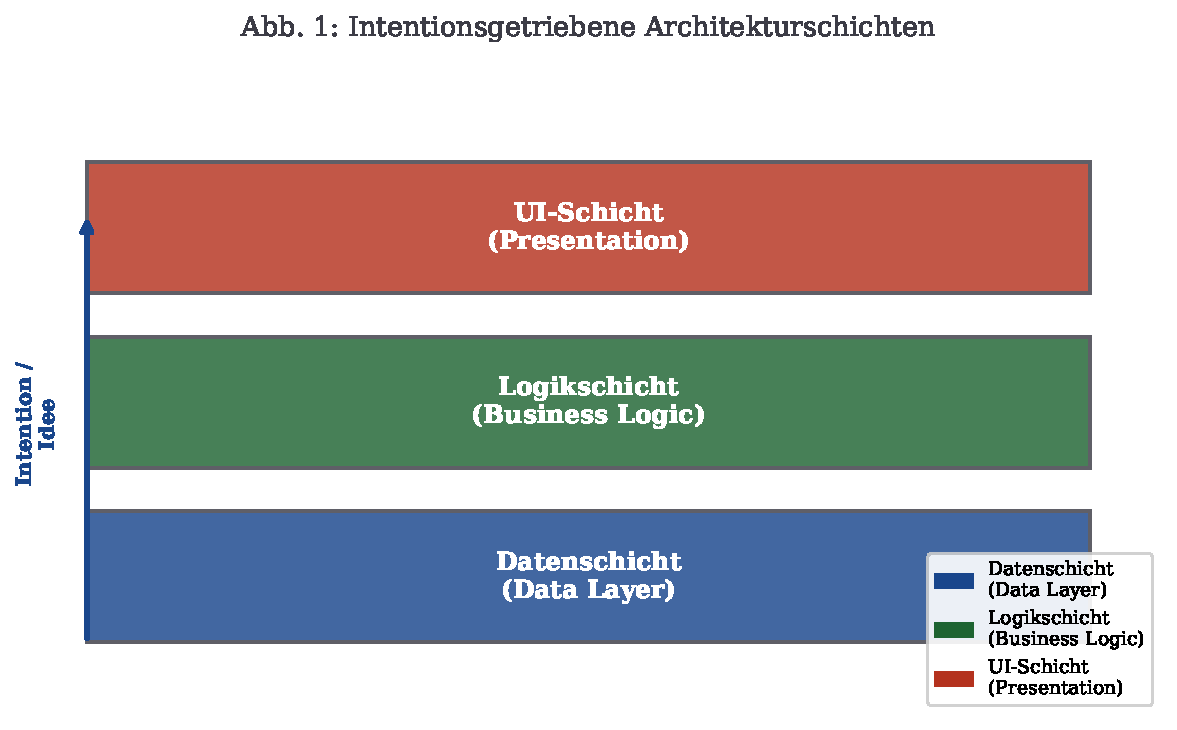
\includegraphics[width=0.82\textwidth]{plot1_architekturschichten.pdf}
    \caption{Intentionsgetriebene Architekturschichten. Der Pfeil links
    symbolisiert die durchgängige Wirkkraft der Leitintention $\mathcal{I}$
    von der Datenschicht bis zur UI-Schicht.}
    \label{fig:architekturschichten}
\end{figure}

% ============================================================
\section{Formale Ergebnisse: Grundmodell}
% ============================================================

\subsection{Das Intentionsprinzip}

\begin{prinzip}[Intentionsprinzip]\label{prinzip:intention}
Der Erfinder oder Entwickler des Softwaresystems treibt die Entwicklung
intentions- oder ideen-getrieben bis zur Reife konsequent und konservativ.
Die Leitintention $\mathcal{I}$ treibt den Entwurf aller Schichten
$\mathcal{D}$, $\mathcal{L}$ und $\mathcal{U}$.
\end{prinzip}

\begin{satz}[Existenz und Eindeutigkeit der Prioritätsfunktion]
\label{satz:existenz}
Zu jeder Leitintention $\mathcal{I} \in \mathbf{I}$ existiert eine
eindeutige Prioritätsfunktion $\Pi(\cdot, \mathcal{I})$, die die
Normierungsbedingung erfüllt und die primäre Schicht $S^*(\mathcal{I})$
korrekt identifiziert.
\end{satz}

\begin{proof}
Wir konstruieren $\Pi$ explizit. Sei $S^*(\mathcal{I})$ die primäre
Schicht und $S^{**}(\mathcal{I})$ die sekundäre. Dann setze:
\begin{align}
\Pi(S^*, \mathcal{I}) &= p^* \in (1/3, 1), \\
\Pi(S^{**}, \mathcal{I}) &= p^{**} \in (0, p^*), \\
\Pi(S^{\circ}, \mathcal{I}) &= 1 - p^* - p^{**} > 0,
\end{align}
wobei $S^{\circ}$ die verbleibende Schicht ist. Die Normierungsbedingung
ist per Konstruktion erfüllt. Die Positivität aller drei Terme folgt
aus $p^* > 1/2$ und $p^{**} > (1-p^*)/2 > 0$. Die Eindeutigkeit
folgt daraus, dass $S^*$ durch die Intention eindeutig bestimmt ist.
\end{proof}

\begin{bemerkung}
Jede Schicht -- auch die mit niedrigster Priorität -- erhält stets einen
strikt positiven Beitrag. Dies entspricht genau dem Leitgedanken: Auch
wenn die UI-Schicht nicht die höchste Priorität hat, hat sie dennoch
besondere Bedeutung zum Zugang der effizienten Datenstruktur.
\end{bemerkung}

\subsection{UI-Primat, Daten-Primat und Logik-Primat}

\begin{satz}[UI-Primat]\label{satz:uiprimat}
Sei $\mathcal{I}_{UI}$ eine UI-Primat-Intention. Dann gilt:
(1) $\Pi(\mathcal{U}, \mathcal{I}_{UI}) > 1/3$.
(2) $\Pi(\mathcal{D}), \Pi(\mathcal{L}) > 0$.
(3) Die Datenschicht und Logikschicht sind notwendige Bedingungen
für die Realisierbarkeit der UI-Intention.
\end{satz}

\begin{proof}
(1) folgt aus UI-Primat-Definition und Normierung.
(2) aus der Normierungsbedingung mit Positivität.
(3) Formal gilt: $\rho(t) \to 1$ erfordert $\Pi(S) > 0$ für alle $S$,
da $\lim_{\Pi(\mathcal{D}) \to 0} \rho = 0$.
\end{proof}

\begin{satz}[Daten-Primat]\label{satz:datenprimat}
Sei $\mathcal{I}_{D}$ eine Daten-Primat-Intention. Dann gilt:
(1) $\Pi(\mathcal{D}, \mathcal{I}_{D}) > 1/3$.
(2) Die UI-Schicht ist das notwendige Tor zur effizienten
Datenstruktur: $A(\mathcal{D}, t) = f(\Pi(\mathcal{U}))$ mit
$f$ streng monoton wachsend und $f(0) = 0$.
(3) $\Pi(\mathcal{U}, \mathcal{I}_{D}) > 0$.
\end{satz}

\begin{proof}
Symmetrisch zu Satz~\ref{satz:uiprimat}. Aussage (2) folgt aus der
Nutzungsbedingung: Ohne UI-Zugang ist die effiziente Datenstruktur
für den Nutzer nicht erreichbar.
\end{proof}

\begin{figure}[h]
    \centering
    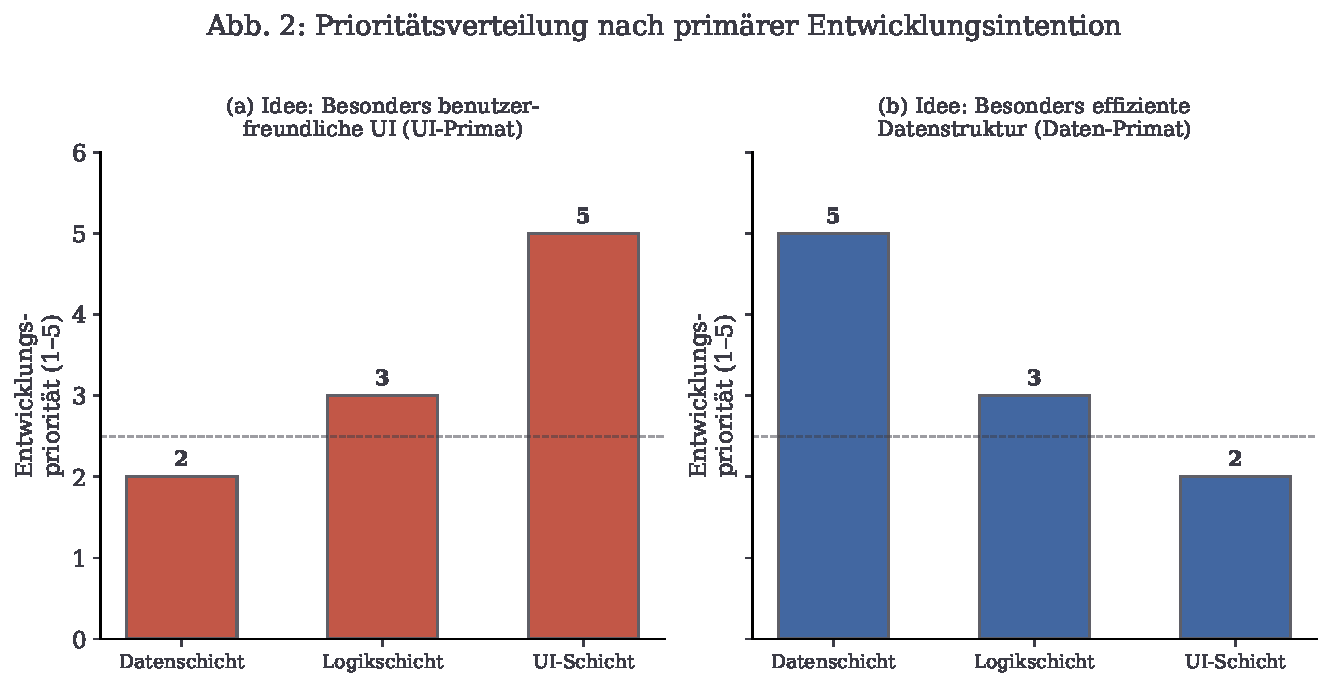
\includegraphics[width=0.92\textwidth]{plot2_prioritaetsverteilung.pdf}
    \caption{Prioritätsverteilung nach primärer Entwicklungsintention.
    Links: UI-Primat ($\mathcal{I}_{UI}$), rechts: Daten-Primat
    ($\mathcal{I}_D$). In beiden Fällen erhalten alle drei Schichten
    einen positiven Prioritätswert.}
    \label{fig:prioritaet}
\end{figure}

\subsection{Konsequenz, Reife und Kosten}

\begin{prinzip}[Konsequenz-Konservativitäts-Prinzip]\label{prinzip:konsequenz}
In allen Fällen -- ob UI-Primat, Daten-Primat, Logik-Primat oder jede
andere Intentionsform -- ist die konsequente und konservative Entwicklung
das entscheidende Qualitätsmerkmal. Für dieses eine Ziel oder diese eine
Erfindung oder Idee wird oder wurde das System entwickelt.
\end{prinzip}

\begin{satz}[Monotonie der Reife unter Konsequenz]\label{satz:monotonie}
Sei $\kappa \equiv \text{const}$. Dann gilt:
\[
\rho(t) = \frac{1}{1 + e^{-\lambda(\kappa)(t - t_{1/2})}},
\]
mit $\lambda(\kappa)$ streng wachsend in $\kappa$. Die Reife ist
eine streng monoton wachsende Funktion der Zeit.
\end{satz}

\begin{proof}
Die Reifungsdynamik erfüllt die logistische Differentialgleichung:
\[
\dot{\rho}(t) = \lambda(\kappa) \cdot \rho(t) \cdot (1 - \rho(t)).
\]
Durch Separation der Variablen:
\[
\int \frac{d\rho}{\rho(1-\rho)} = \lambda(\kappa) \int dt
\implies \rho(t) = \frac{1}{1 + e^{-\lambda(\kappa)(t - t_{1/2})}}.
\]
Strenge Monotonie: $\dot{\rho}(t) > 0$ für alle $t$, da
$\lambda(\kappa) > 0$ und $\rho \in (0,1)$. Da $\lambda$ streng
wächst, beschleunigt höhere Konsequenz die Reifung.
\end{proof}

\begin{figure}[h]
    \centering
    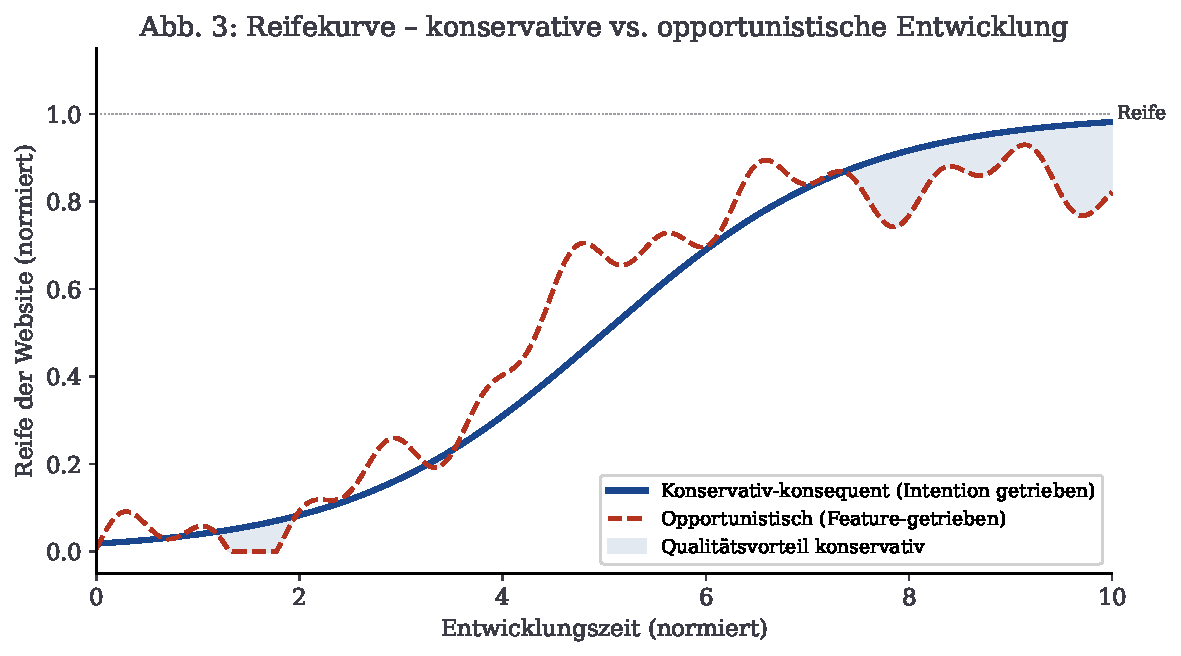
\includegraphics[width=0.88\textwidth]{plot3_reifekurve.pdf}
    \caption{Reifekurve: Konservativ-konsequente Entwicklung (blau)
    folgt einem glatten sigmoiden Verlauf. Opportunistische Entwicklung
    (rot, gestrichelt) zeigt Oszillationen durch häufige Richtungswechsel.}
    \label{fig:reifekurve}
\end{figure}

\begin{lemma}[Superlinearität der Inkonsistenzkosten]\label{lem:kosten}
Für eine konsequente Entwicklung gilt $K_{\kappa=1}(t) = a + bt$
(linear). Für $\kappa < 1$ gilt:
\[
K_{\kappa}(t) = a + \beta t + \delta(\kappa) \cdot t^2,
\quad \delta(\kappa) = \frac{c \mu (1 - \kappa)}{2} > 0.
\]
Jede Inkonsistenz erzeugt superlineare (quadratische) Mehrkosten.
\end{lemma}

\begin{proof}
Inkonsistente Entwicklung erfordert Refactoring-Iterationen mit Rate
$\mu(1-\kappa)$. Die kumulativen Refactoring-Kosten bis $t$:
\[
K_{\text{ref}}(t) = c \int_0^t \mu(1-\kappa) s \, ds
= \frac{c \mu (1-\kappa)}{2} \cdot t^2 = \delta(\kappa) \cdot t^2.
\]
$\delta'(\kappa) = -c\mu/2 < 0$: Je konsequenter, desto geringer
die quadratischen Kosten. Für $\kappa = 1$: $\delta(1) = 0$.
\end{proof}

\begin{figure}[h]
    \centering
    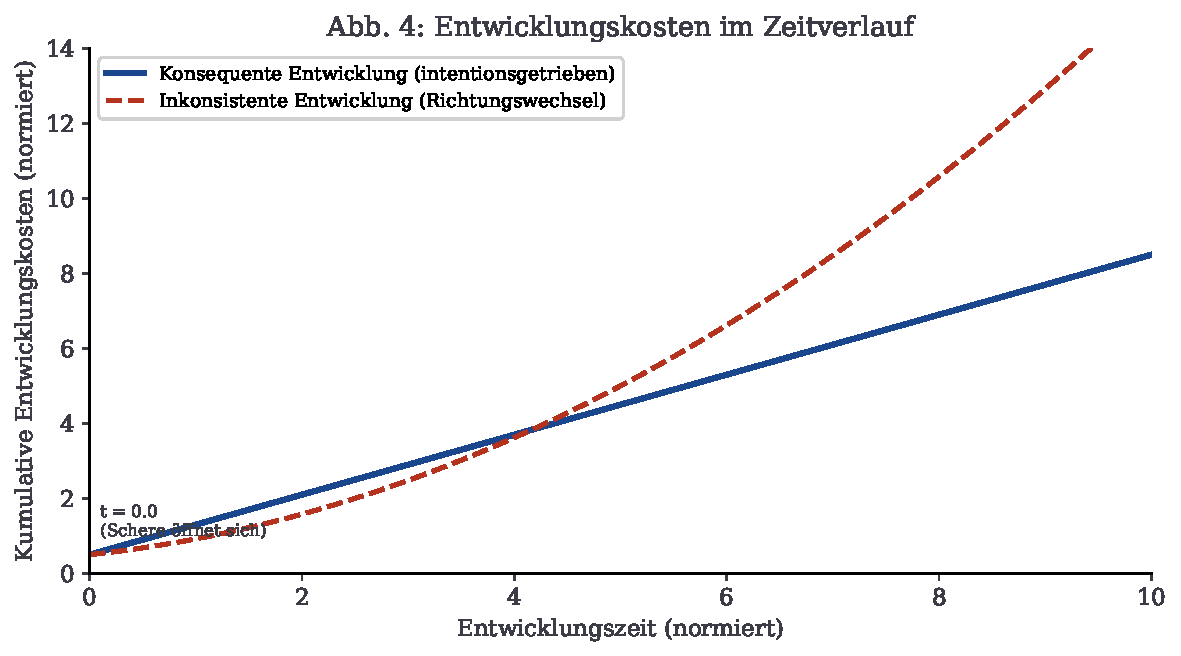
\includegraphics[width=0.88\textwidth]{plot4_entwicklungskosten.pdf}
    \caption{Entwicklungskosten: Konsequente Entwicklung (blau) wächst
    linear; inkonsistente Entwicklung (rot) wächst quadratisch durch
    kumulative Refactoring-Kosten (Lemma~\ref{lem:kosten}).}
    \label{fig:kosten}
\end{figure}

\subsection{Kohärenz- und Qualitätssätze}

\begin{satz}[Schichten-Kohärenz-Theorem]\label{satz:kohärenz}
Für jede Schicht $S$: (1) $\gamma_S(\kappa)$ ist streng monoton
wachsend. (2) $\gamma_S(0) = 0$. (3) $\gamma_S(1) = c_S$.
(4) Die Interschicht-Kohärenz $\Gamma(\kappa) = \min_S \gamma_S(\kappa)$
ist ebenfalls streng monoton wachsend in $\kappa$.
\end{satz}

\begin{proof}
(1) $\gamma_S'(\kappa) = c_S \alpha_S \kappa^{\alpha_S-1} > 0$.
(2) $\gamma_S(0) = 0$. (3) $\gamma_S(1) = c_S$.
(4) Minimum streng monotoner Funktionen ist streng monoton.
\end{proof}

\begin{figure}[h]
    \centering
    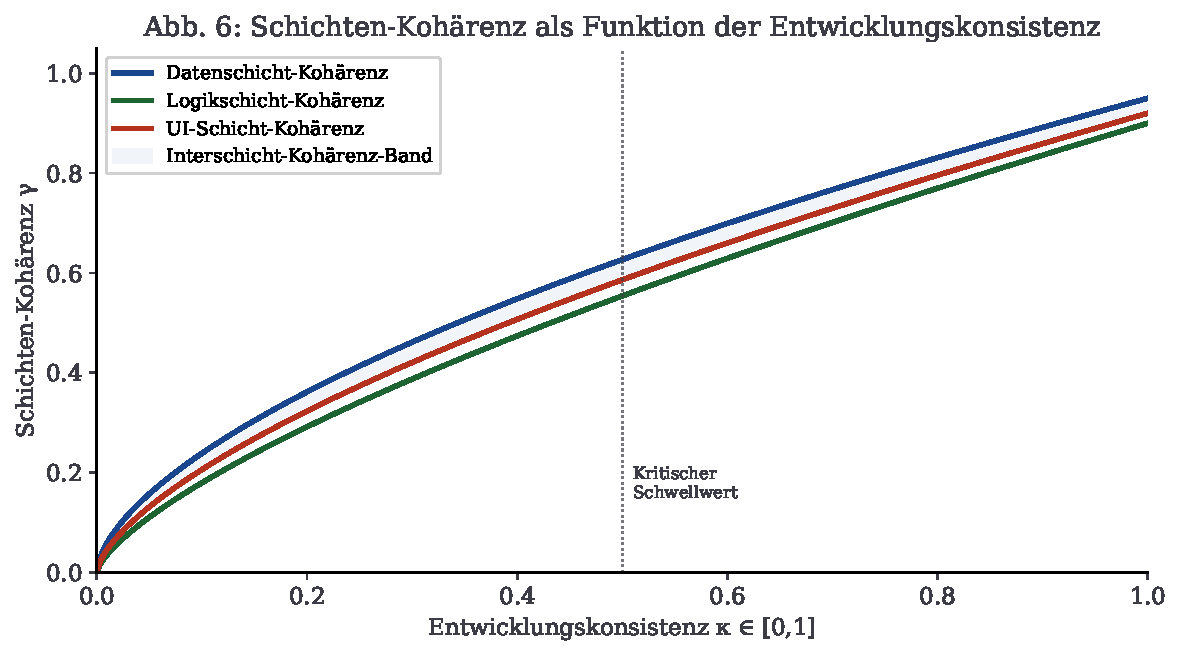
\includegraphics[width=0.88\textwidth]{plot6_kohaerenz.pdf}
    \caption{Schichten-Kohärenz als Funktion der Konsistenz $\kappa$.
    Alle Schichten zeigen streng monoton wachsende Kohärenz.}
    \label{fig:kohärenz}
\end{figure}

\begin{satz}[Qualitätsvorteil konservativer Entwicklung]\label{satz:qualitaet}
Mit dem Qualitätsmaß $Q(t) = \sum_S \Pi(S, \mathcal{I}) \cdot
\gamma_S(\kappa(t))$ gilt:
\[
Q_{\text{konservativ}}(t) \geq Q_{\text{opportunistisch}}(t)
\quad \forall t > 0.
\]
\end{satz}

\begin{proof}
Konservative Entwicklung hält $\kappa(t) \equiv \kappa_{\max} \approx 1$.
Opportunistische Entwicklung zeigt schwankende Konsistenz mit
$\mathbb{E}[\hat{\kappa}(t)] < \kappa_{\max}$. Da $Q(\cdot)$ eine
positive Linearkombination konvexer Funktionen ist, folgt mit der
Jensen-Ungleichung:
\[
Q(\kappa_{\max}) > Q(\mathbb{E}[\hat{\kappa}]) \geq \mathbb{E}[Q(\hat{\kappa})].
\]
\end{proof}

\begin{figure}[h]
    \centering
    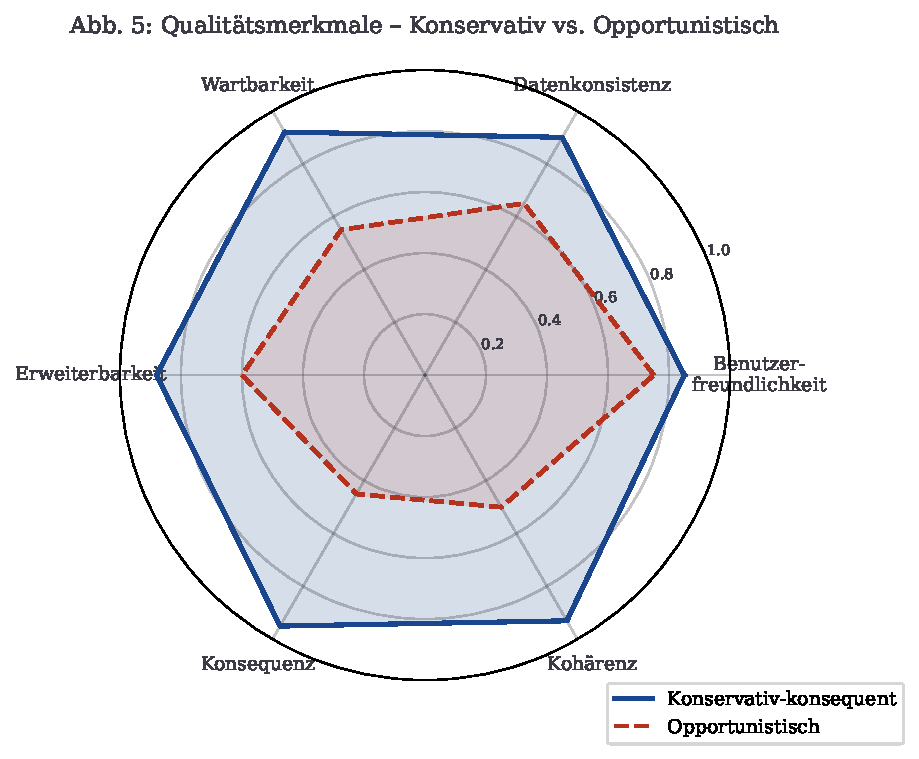
\includegraphics[width=0.72\textwidth]{plot5_radar_qualitaet.pdf}
    \caption{Qualitätsmerkmale im Vergleich: Konsequente Entwicklung (blau)
    übertrifft opportunistische Entwicklung (rot) in allen sechs Dimensionen.}
    \label{fig:radar}
\end{figure}

\begin{satz}[Dualität und Universalität]\label{satz:dualitaet}
Sowohl UI-Primat, Daten-Primat, Logik-Primat als auch alle anderen
Intentionsformen sind spezielle Ausprägungen desselben
Intentionsprinzips. Der Qualitätsvorteil konsequenter Entwicklung
gilt universell, unabhängig von der Wahl der Prioritätsfunktion.
\end{satz}

\begin{proof}
$Q(t) = \sum_S \Pi(S) \gamma_S(\kappa)$ ist eine positive Linearkombination
konvexer Funktionen für jedes beliebige normierte $\Pi$. Daher gilt
Satz~\ref{satz:qualitaet} für alle $\mathcal{I} \in \mathbf{I}$.
\end{proof}

\begin{korollar}[Universalität der Konsequenz]
Für jede Intention $\mathcal{I}$ und $\kappa > 0$:
\[
\frac{\partial Q}{\partial \kappa} =
\sum_S \Pi(S) c_S \alpha_S \kappa^{\alpha_S - 1} > 0.
\]
Konsequenz zahlt sich immer aus.
\end{korollar}

% ============================================================
\section{Verallgemeinerung: Das Paradigma für alle Softwaresysteme}
% ============================================================

Der Leitgedanke des Intentionsprinzips wurde im vorigen Abschnitt für
Websites hergeleitet. In diesem Kernkapitel wird gezeigt, dass er mit
gleicher Kraft für \emph{alle} relevanten Klassen von Softwaresystemen
gilt: mobile Apps, Desktop-Anwendungen, eingebettete Systeme und
verteilte Systeme. Die Verallgemeinerung ist nicht trivial, denn jede
Systemklasse hat eigene technische Constraints, eigene Schichtenstrukturen
und eigene Manifestationen der drei Architekturschichten. Es wird in
jedem Fall gezeigt, dass das Intentionsprinzip (Prinzip~\ref{prinzip:intention})
und das Konsequenz-Konservativitäts-Prinzip (Prinzip~\ref{prinzip:konsequenz})
strukturell invariant bleiben.

Abbildung~\ref{fig:plattformvergleich} gibt einen ersten quantitativen
Ãœberblick: Ãœber alle Plattformen hinweg erzielt konsequente Entwicklung
einen deutlichen und konsistenten Qualitätsvorteil.

\begin{figure}[h]
    \centering
    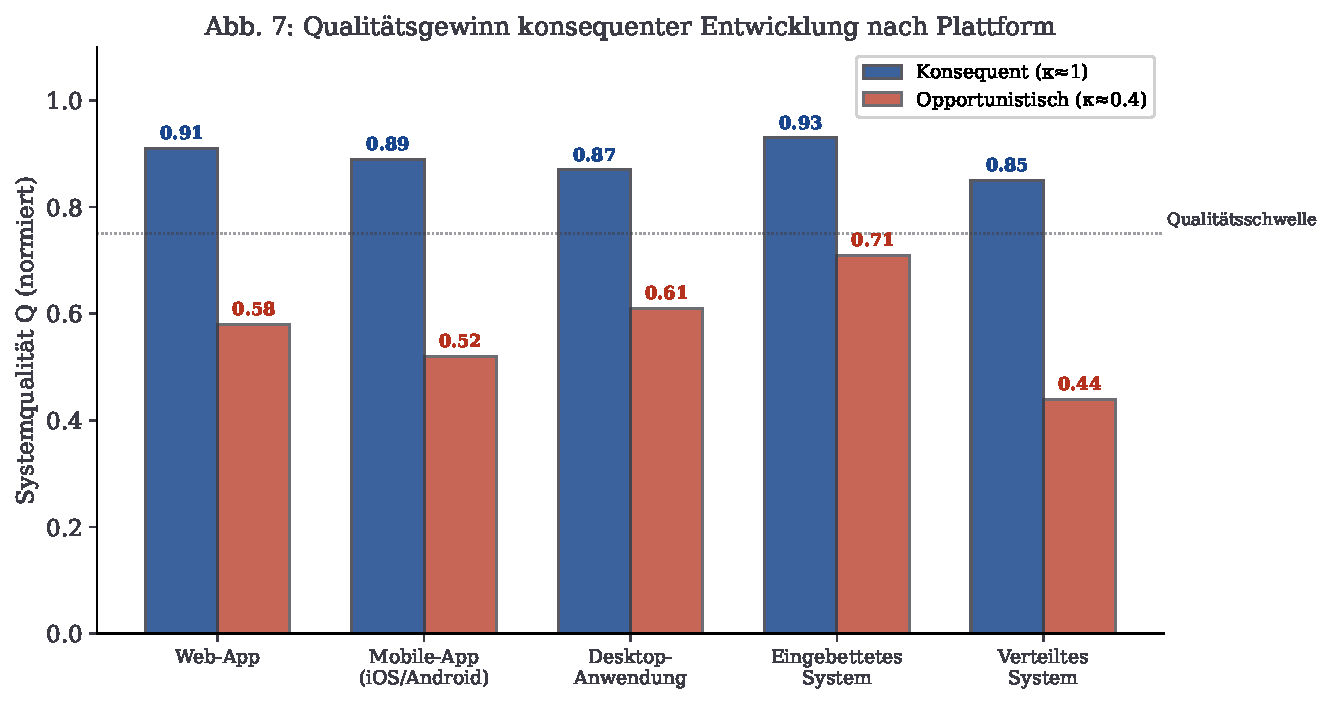
\includegraphics[width=0.96\textwidth]{plot7_plattformvergleich.pdf}
    \caption{Systemqualität $Q$ im Vergleich zwischen konsequenter
    ($\kappa \approx 1$) und opportunistischer ($\kappa \approx 0.4$)
    Entwicklung nach Plattformklasse. In allen Klassen übertrifft
    konsequente Entwicklung die opportunistische deutlich.}
    \label{fig:plattformvergleich}
\end{figure}

\subsection{Mobile App-Entwicklung (iOS und Android)}

\subsubsection{Architekturspezifik mobiler Systeme}

Mobile Apps weisen gegenüber Websites spezifische Constraints auf, die
die Ausprägung der drei Schichten maßgeblich beeinflussen:

\begin{itemize}
    \item \textbf{Ressourcenbeschränkung}: RAM, CPU und Akkukapazität
          sind begrenzt. Jede unnötige Schicht verbraucht wertvolle Ressourcen.
    \item \textbf{Offline-Fähigkeit}: Mobile Apps müssen häufig ohne
          Netzwerkverbindung funktionieren. Die Datenschicht muss daher
          oft lokal (SQLite, Room, Core Data) und synchronisierend zugleich sein.
    \item \textbf{Lifecycle-Komplexität}: Apps können vom Betriebssystem
          jederzeit in den Hintergrund versetzt oder beendet werden.
          Die Logikschicht muss Zustandswiederherstellung unterstützen.
    \item \textbf{Plattformdivergenz}: iOS und Android haben unterschiedliche
          UI-Paradigmen (UIKit/SwiftUI vs. View/Jetpack Compose), was
          bei plattformübergreifender Entwicklung (Flutter, React Native)
          Intentionskonsistenz besonders herausfordernd macht.
\end{itemize}

Trotz dieser Constraints gilt das Intentionsprinzip unverändert. Die
drei Architekturschichten sind:

\begin{itemize}
    \item $\mathcal{D}^{\text{mob}}$: Lokale Datenbank (SQLite, Core
          Data, Realm), Netzwerk-Cache, SharedPreferences/UserDefaults.
    \item $\mathcal{L}^{\text{mob}}$: ViewModels (MVVM), Presenter (MVP),
          Use-Cases (Clean Architecture), Repository-Pattern.
    \item $\mathcal{U}^{\text{mob}}$: Activities/Fragments (Android),
          UIViewControllers/SwiftUI-Views (iOS), Jetpack Compose.
\end{itemize}

\subsubsection{Formale Ãœbertragung des Intentionsprinzips}

\begin{satz}[Intentionsprinzip für mobile Apps]\label{satz:mobile}
Das Intentionsprinzip (Prinzip~\ref{prinzip:intention}) gilt für mobile
Apps mit den Schichten $\mathcal{D}^{\text{mob}}$,
$\mathcal{L}^{\text{mob}}$, $\mathcal{U}^{\text{mob}}$.
Insbesondere: Jede Architekturentscheidung für eine mobile App --
ob Datenbankschema, Repository-Pattern oder UI-Komponentenstruktur --
muss sich aus der Leitintention $\mathcal{I}$ ableiten lassen.
\end{satz}

\begin{proof}
Die formale Struktur ist identisch zur Web-Version: Die Normierungsbedingung,
die Positivitätsbedingung und der Konsequenz-Koeffizient $\kappa$ sind
plattformunabhängig definiert (Definition~5 und~8). Die Existenz der
drei Schichten $\mathcal{D}^{\text{mob}}$, $\mathcal{L}^{\text{mob}}$,
$\mathcal{U}^{\text{mob}}$ in jeder mobilen App (unabhängig von der
verwendeten Architektur MVC, MVP, MVVM oder Clean Architecture) ist
eine empirische Tatsache, die durch sämtliche offiziellen Architektur-
richtlinien von Google (Android Architecture) und Apple (UIKit/SwiftUI)
bestätigt wird \cite{google2023architecture, apple2023swiftui}.
Damit sind alle Voraussetzungen der Sätze \ref{satz:existenz}--\ref{satz:dualitaet}
auf mobile Systeme übertragbar.
\end{proof}

\begin{beispiel}[Sofort-Kamera-App -- UI-Primat]\label{bsp:kamera}
Eine Entwicklerin entwirft eine Kamera-App für iOS mit der Leitintention
$\mathcal{I}_{UI}$: \textit{\glqq{}Ein Foto soll in unter zwei Sekunden vom
Entsperren des Telefons bis zur Aufnahme erreichbar sein.\grqq{}} Diese
UI-Primat-Intention strukturiert alle Entscheidungen:

\begin{center}
\begin{tabular}{lcp{5.5cm}}
\toprule
Schicht & $\Pi(S)$ & Entwurfsentscheidung \\
\midrule
UI ($\mathcal{U}^{\text{mob}}$) & 0.65 & Lock-Screen-Widget, minimale
Gesten, sofortiger Kamerastart ohne Lade-Bildschirm \\
Logik ($\mathcal{L}^{\text{mob}}$) & 0.25 & Schneller Autofokus-Algorithmus,
Bildvorverarbeitung im Hintergrund \\
Daten ($\mathcal{D}^{\text{mob}}$) & 0.10 & Asynchrones Schreiben in die
Fotobibliothek, kein blockierender Schreibvorgang \\
\bottomrule
\end{tabular}
\end{center}

Inkonsistenz-Warnung: Das Hinzufügen eines komplexen Foto-Filter-Editors
(UI-Umbau), eines KI-Bilderkennungs-Backends (Logik-Primat) oder einer
iCloud-Synchronisation (Daten-Priorität) -- ohne Anpassung der
Leitintention -- würde $\kappa$ auf unter 0.5 senken und gemäß
Lemma~\ref{lem:kosten} quadratische Mehrkosten erzeugen.
\end{beispiel}

\begin{beispiel}[Offline-First-Sync-App -- Daten-Primat]\label{bsp:sync}
Ein Team entwickelt eine Feldvermessungs-App für Android, die ohne
Mobilfunknetz funktionieren muss. Leitintention $\mathcal{I}_D$:
\textit{\glqq{}Alle Messdaten werden zuverlässig gespeichert und bei
Netzwerkverbindung vollständig und konfliktfrei synchronisiert.\grqq{}}

\begin{center}
\begin{tabular}{lcp{5.5cm}}
\toprule
Schicht & $\Pi(S)$ & Entwurfsentscheidung \\
\midrule
Daten ($\mathcal{D}^{\text{mob}}$) & 0.60 & Room + WorkManager, CRDT-basierte
Konfliktauflösung, SQLite WAL-Modus \\
Logik ($\mathcal{L}^{\text{mob}}$) & 0.30 & Repository-Pattern,
Synchronisations-Scheduler, Delta-Sync-Algorithmus \\
UI ($\mathcal{U}^{\text{mob}}$) & 0.10 & Schlichtes Formular-Interface,
Sync-Status-Anzeige \\
\bottomrule
\end{tabular}
\end{center}

Gemäß Satz~\ref{satz:datenprimat} erhält die UI-Schicht $\Pi = 0.10 > 0$:
Sie ist das notwendige Tor zu den Messdaten für den Feldvermesser --
ohne sie wären die zuverlässig gespeicherten Daten im Feld nicht erfassbar.
\end{beispiel}

\begin{figure}[h]
    \centering
    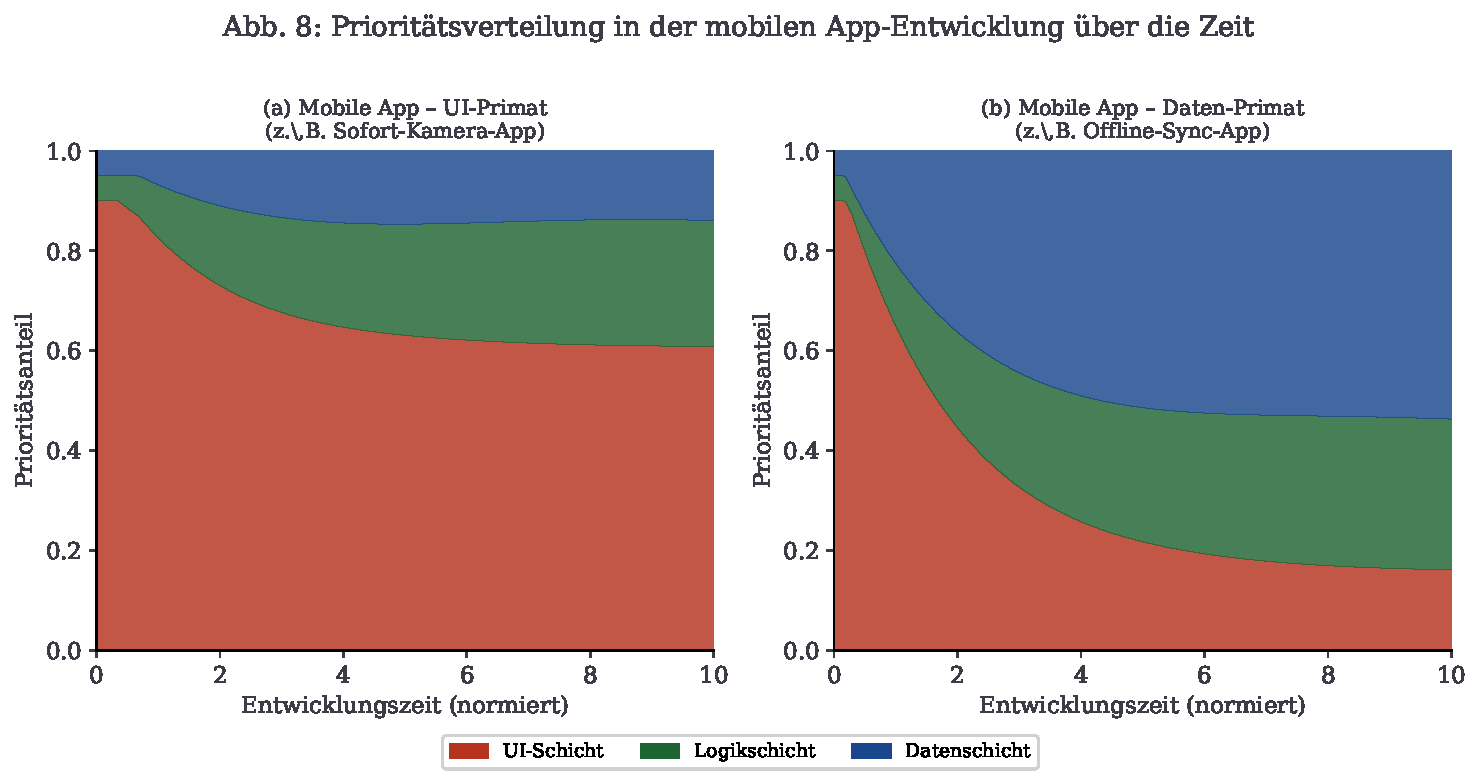
\includegraphics[width=0.96\textwidth]{plot8_mobile_prioritaet.pdf}
    \caption{Prioritätsverteilung in der mobilen App-Entwicklung über
    die Zeit. Links: UI-Primat (Sofort-Kamera-App). Rechts: Daten-Primat
    (Offline-Sync-App). In beiden Fällen pendeln sich die Prioritäten
    auf die intentionskonsistente Verteilung ein.}
    \label{fig:mobile}
\end{figure}

\subsubsection{Plattformübergreifende Entwicklung und Intentionskonsistenz}

Plattformübergreifende Frameworks wie Flutter oder React Native stellen
eine besondere Herausforderung für das Intentionsprinzip dar. Sie versprechen
eine einzige Codebasis für iOS und Android, erzeugen aber häufig eine
vierte, implizite Schicht -- den Plattform-Abstraktionskanal --
die die Intentionskonsistenz gefährden kann.

\begin{lemma}[Plattform-Abstraktion und Konsequenz]\label{lem:plattform}
Sei $\mathcal{A}$ ein Plattform-Abstraktionskanal (Flutter Engine,
React Native Bridge). Dann gilt: Der Konsequenz-Koeffizient $\kappa$
des Gesamtsystems ist nach oben beschränkt durch:
\[
\kappa_{\text{gesamt}} \leq \kappa_{\text{App}} \cdot \eta(\mathcal{A}),
\]
wobei $\eta(\mathcal{A}) \in (0, 1]$ die Intentionstreue des Abstraktions-
kanals bezeichnet: $\eta = 1$ bei perfekter Plattformintegration,
$\eta < 1$ bei plattformspezifischen Brüchen.
\end{lemma}

\begin{proof}
Jede Inkonsistenz, die durch die Plattform-Abstraktion eingeführt wird
(z.\,B. unterschiedliches Look-and-Feel zwischen iOS und Android trotz
einheitlichem Code), reduziert den effektiven Konsequenz-Koeffizienten.
Formal: Wenn $\mathcal{A}$ mit Wahrscheinlichkeit $1 - \eta$ eine
Entwurfsentscheidung plattforminkonsistent darstellt, dann folgt
aus dem Produktsatz der Wahrscheinlichkeiten die obige Schranke.
\end{proof}

\subsection{Desktop-Anwendungen}

\subsubsection{Architekturspezifik von Desktop-Systemen}

Desktop-Anwendungen (Windows, macOS, Linux -- nativ oder mit Electron/Qt)
unterscheiden sich von Web- und mobilen Apps in mehreren relevanten Aspekten:

\begin{itemize}
    \item \textbf{Reichere Ressourcen}: Desktop-Systeme haben in der Regel
          mehr RAM, CPU und persistenten Speicher zur Verfügung. Dies vergrößert
          den Raum der möglichen Entwurfsentscheidungen und damit auch das
          Risiko, die Leitintention durch unnötige Komplexität zu verwässern.
    \item \textbf{Komplexere UI-Paradigmen}: Drag-and-Drop, Kontextmenüs,
          Tastaturkürzel, Menüleisten -- Desktop-UIs sind reichhaltiger.
          Dies kann dazu verführen, UI-Features zu ergänzen, die nicht der
          Leitintention dienen.
    \item \textbf{Interprozesskommunikation}: Desktop-Apps interagieren
          häufig mit dem Betriebssystem, anderen Prozessen und Hardware-
          peripherie. Jede Schnittstelle ist eine potenzielle Quelle von
          Inkonsistenz.
\end{itemize}

\begin{definition}[Desktop-Schichtenmodell]
Für Desktop-Anwendungen sind die drei Architekturschichten:
$\mathcal{D}^{\text{desk}}$ (lokale Datei- und Datenbanksysteme, ORM,
Konfigurationspersistenz),
$\mathcal{L}^{\text{desk}}$ (Geschäftslogik, Controller, Presenter,
Hintergrundverarbeitung, Plugins),
$\mathcal{U}^{\text{desk}}$ (nativer UI-Toolkit, Fensterverwaltung,
Event-Loop, Widgets).
\end{definition}

\begin{satz}[Intentionsprinzip für Desktop-Anwendungen]\label{satz:desktop}
Das Intentionsprinzip gilt für Desktop-Anwendungen mit den Schichten
$\mathcal{D}^{\text{desk}}$, $\mathcal{L}^{\text{desk}}$,
$\mathcal{U}^{\text{desk}}$. Für Desktop-Anwendungen mit reicheren
Ressourcen gilt darüber hinaus: Die erhöhte Ressourcenverfügbarkeit
erhöht ceteris paribus das Risiko der Intentionsverwässerung, da
mehr Entwurfsentscheidungen möglich sind.
\end{satz}

\begin{proof}
Die erste Aussage folgt aus der plattformunabhängigen Formulierung von
Prinzip~\ref{prinzip:intention}. Für die zweite Aussage: Sei $N(r)$
die Anzahl der möglichen Entwurfsentscheidungen als wachsende Funktion
der verfügbaren Ressourcen $r$. Dann ist die Wahrscheinlichkeit einer
zufälligen intentionsfremden Entscheidung:
\[
P_{\text{inkonsequent}} = \frac{N_{\text{fremd}}(r)}{N(r)}.
\]
Da $N_{\text{fremd}}(r)$ schneller wächst als $N_{\text{konform}}(r)$
(mehr Ressourcen eröffnen überproportional mehr nicht-intentionskonforme
Möglichkeiten), steigt das Verwässerungsrisiko. Konsequenz ist daher
bei ressourcenreichen Systemen noch wichtiger.
\end{proof}

\begin{beispiel}[Texteditor -- Logik-Primat]\label{bsp:texteditor}
Ein Entwickler entwirft einen Texteditor für Programmierer mit der
Leitintention $\mathcal{I}_L$: \textit{\glqq{}Der Editor führt jede
Benutzeraktion in unter 16\,ms aus (60\,fps, keine spürbaren Pausen).\grqq{}}
Dies ist eine Logik-Primat-Intention: Nicht die visuelle Gestaltung,
sondern die algorithmische Kernleistung steht im Vordergrund.

\begin{center}
\begin{tabular}{lcp{5.5cm}}
\toprule
Schicht & $\Pi(S)$ & Entwurfsentscheidung \\
\midrule
Logik ($\mathcal{L}^{\text{desk}}$) & 0.55 & Piece-Table-Datenstruktur,
inkrementelles Syntaxhighlighting, asynchrone Sprachserverprotokolle \\
Daten ($\mathcal{D}^{\text{desk}}$) & 0.30 & Memory-Mapped Files, lazy
loading, kein blockierendes Schreiben \\
UI ($\mathcal{U}^{\text{desk}}$) & 0.15 & Schlichtes Monospace-Rendering,
minimale Animationen \\
\bottomrule
\end{tabular}
\end{center}

Konsequenz-Gefahr: Das Hinzufügen von Markdown-Preview-Rendering (hohe
UI-Komplexität), Plugin-Scripting (Logik-Erweiterung) oder Cloud-Sync
(Daten-Umbau) -- ohne Anpassung der Performance-Intention -- würde
$\kappa$ senken und die 16\,ms-Garantie gefährden.
\end{beispiel}

\subsection{Eingebettete Systeme}

\subsubsection{Architekturspezifik eingebetteter Systeme}

Eingebettete Systeme (Mikrocontroller, FPGAs, industrielle Steuerungen,
IoT-Devices) stellen die härtesten Anforderungen an Konsequenz, denn:

\begin{itemize}
    \item \textbf{Ressourcenextremum}: Typische Mikrocontroller haben
          wenige Kilobytes RAM und hunderte Kilobytes Flash. Jede Byte,
          das durch intentionsfremde Features belegt wird, fehlt dem
          Kernsystem.
    \item \textbf{Harte Echtzeitanforderungen}: Verletzungen der
          Leitintention können direkte physikalische Konsequenzen haben
          (Motorausfall, Sicherheitsversagen, Datenverlust).
    \item \textbf{Fehlende Laufzeitflexibilität}: In Gegensatz zu Web-
          oder Desktop-Systemen kann eine eingebettete Firmware nicht
          einfach gepatcht werden. Inkonsequente Entwurfsentscheidungen
          verursachen extrem hohe Rückruf- und Nachbesserungskosten.
    \item \textbf{Physikalische Nähe}: Die UI-Schicht manifestiert sich
          als Sensorschnittstellen, Aktuatoren, Displays oder Feldbusse
          (CAN, Modbus, EtherCAT).
\end{itemize}

\begin{definition}[Embedded-Schichtenmodell]
Für eingebettete Systeme sind die Architekturschichten:
$\mathcal{D}^{\text{emb}}$ (nichtflüchtiger Speicher: EEPROM, Flash,
SD-Karte; Ringpuffer, Sensorpuffer),
$\mathcal{L}^{\text{emb}}$ (Steuerungsalgorithmen, Echtzeitscheduler,
Kommunikationsprotokolle, Treiberschicht),
$\mathcal{U}^{\text{emb}}$ (Aktuatoren, Feldbusse, Displays, LEDs,
externe Kommunikationsinterfaces).
\end{definition}

\begin{satz}[Intentionsprinzip für eingebettete Systeme]\label{satz:embedded}
Das Intentionsprinzip gilt für eingebettete Systeme mit den Schichten
$\mathcal{D}^{\text{emb}}$, $\mathcal{L}^{\text{emb}}$,
$\mathcal{U}^{\text{emb}}$. Der Quadratkoeffizient der Inkonsistenzkosten
(Lemma~\ref{lem:kosten}) ist für eingebettete Systeme um den Faktor
\[
\delta_{\text{emb}} = \delta_{\text{web}} \cdot F_{\text{field}},
\quad F_{\text{field}} \gg 1,
\]
erhöht, wobei $F_{\text{field}}$ die Feldrückruf-Kostenmultiplikation
bezeichnet.
\end{satz}

\begin{proof}
Für eingebettete Systeme, die in der Produktion verbaut sind, erfordert
eine inkonsequente Entwurfsentscheidung nicht nur Softwarerefactoring,
sondern potenziell Hardware-Revisionen, Feldservice-Einsätze und
Produktrückrufe. Sei $C_{\text{field}}$ die durchschnittlichen Kosten
eines Feldservice-Einsatzes und $n_{\text{units}}$ die Anzahl der
verbauten Einheiten, dann gilt:
\[
\delta_{\text{emb}} = \delta_{\text{web}} + \frac{c_{\text{field}} \cdot
n_{\text{units}}}{T^2_{\text{ref}}},
\]
wobei $T_{\text{ref}}$ der Referenzzeitraum ist. Da
$c_{\text{field}} \cdot n_{\text{units}} \gg 0$ für typische
Feldanwendungen, folgt $F_{\text{field}} \gg 1$.
\end{proof}

\begin{figure}[h]
    \centering
    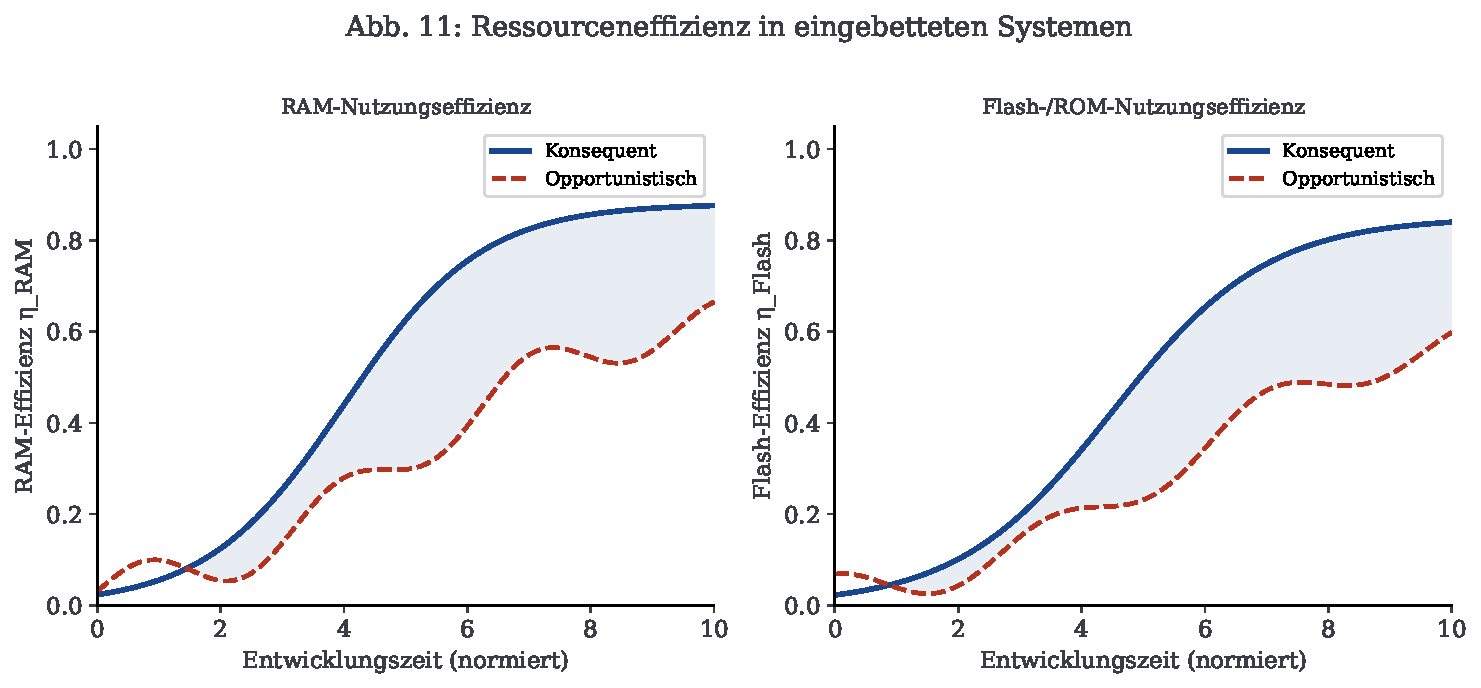
\includegraphics[width=0.96\textwidth]{plot11_embedded_ressourcen.pdf}
    \caption{Ressourceneffizienz in eingebetteten Systemen: Konsequente
    Entwicklung (blau) erzielt signifikant höhere RAM- und Flash-Nutzungs-
    effizienz als opportunistische Entwicklung (rot).}
    \label{fig:embedded}
\end{figure}

\begin{beispiel}[Motorsteuerung -- Logik-Primat]\label{bsp:motor}
Ein Entwickler entwirft eine BLDC-Motorsteuerung auf einem STM32F4
mit der Leitintention $\mathcal{I}_L$: \textit{\glqq{}Der Regelkreis
wird in 100\,$\mu$s mit einer Drehzahlgenauigkeit von $\pm$0.5\,\%
geschlossen.\grqq{}} Alle Schichten dienen dieser Echtzeitintention:

\begin{center}
\begin{tabular}{lcp{5.5cm}}
\toprule
Schicht & $\Pi(S)$ & Entwurfsentscheidung \\
\midrule
Logik ($\mathcal{L}^{\text{emb}}$) & 0.70 & Field-Oriented Control
(FOC), DMA-basierter ADC, Interrupt-driven Scheduling \\
Daten ($\mathcal{D}^{\text{emb}}$) & 0.20 & Ringpuffer für Messwerte,
EEPROM nur für Konfigurationsparameter \\
UI ($\mathcal{U}^{\text{emb}}$) & 0.10 & CAN-Bus Status-Telegramme,
eine Status-LED \\
\bottomrule
\end{tabular}
\end{center}

Intentionsverletzung: Das nachträgliche Hinzufügen eines UART-Debuginter-
faces mit printf-Ausgaben würde die ISR-Latenz erhöhen und die 100\,$\mu$s-
Garantie gefährden -- eine klassische inkonsequente Entwurfsentscheidung.
\end{beispiel}

\subsection{Verteilte Systeme und Microservices}

\subsubsection{Architekturspezifik verteilter Systeme}

Verteilte Systeme -- Microservice-Architekturen, Event-Driven Systems,
Cloud-native Anwendungen -- stellen besondere Herausforderungen an das
Intentionsprinzip, da die drei Architekturschichten über mehrere physische
Knoten verteilt sein können:

\begin{itemize}
    \item \textbf{Schichtenverteilung}: Die Datenschicht kann über mehrere
          Datenbankservices (PostgreSQL, Redis, Cassandra) verteilt sein;
          die Logikschicht über hunderte Microservices; die UI-Schicht über
          Frontend-Services und API-Gateways.
    \item \textbf{CAP-Theorem}: Konsistenz, Verfügbarkeit und
          Partitionstoleranz können nicht gleichzeitig maximiert werden
          \cite{brewer2000cap}. Die Wahl der Leitintention bestimmt, welche
          dieser Eigenschaften priorisiert wird.
    \item \textbf{Conway's Law}: Die Organisationsstruktur des Entwicklungs-
          teams spiegelt sich in der Systemarchitektur wider \cite{conway1968}.
          Teams ohne gemeinsame Leitintention produzieren Architekturen ohne
          Intentionskonsistenz.
    \item \textbf{Verteilte Inkonsistenz}: Inkonsequente Entwurfs-
          entscheidungen in einem Microservice pflanzen sich über APIs auf
          andere Services fort und multiplizieren die Inkonsistenzkosten.
\end{itemize}

\begin{definition}[Verteiltes Schichtenmodell]
Für verteilte Systeme sind die Architekturschichten:
$\mathcal{D}^{\text{dist}}$ (Datenbankcluster, Message Queues, Event
Stores, Distributed Caches),
$\mathcal{L}^{\text{dist}}$ (Microservices, Worker Processes, Saga
Orchestrators, Event Handler),
$\mathcal{U}^{\text{dist}}$ (API Gateway, GraphQL-Layer, Frontend-Services,
Webhooks, CLI-Tools).
\end{definition}

\begin{satz}[Multiplikative Inkonsistenzkosten in verteilten Systemen]
\label{satz:distributed}
In einem verteilten System mit $k$ Microservices gilt für die
Gesamtinkonsistenzkosten:
\[
K_{\text{dist}}(t) = \sum_{i=1}^k K_i(t) +
\sum_{i \neq j} C_{ij} \cdot (1 - \kappa_i)(1 - \kappa_j) \cdot t^2,
\]
wobei $K_i(t)$ die lokalen Inkonsistenzkosten von Service $i$ sind,
$\kappa_i$ sein lokaler Konsequenz-Koeffizient, und $C_{ij} > 0$
die API-Kopplungskosten zwischen Service $i$ und $j$.
\end{satz}

\begin{proof}
Die lokalen Terme $K_i(t)$ folgen aus Lemma~\ref{lem:kosten} für
jeden Service $i$. Die Kopplungsterme entstehen, weil eine inkonsequente
Entscheidung in Service $i$ (mit Wahrscheinlichkeit proportional zu
$1-\kappa_i$) und eine inkonsequente Entscheidung in Service $j$
(proportional zu $1-\kappa_j$), die dieselbe API betreffen, gemeinsam
mit Kosten $C_{ij}$ einen Refactoring-Zyklus erfordern. Die Häufigkeit
solcher gleichzeitiger Inkonsistenzen ist proportional zum Produkt
$(1-\kappa_i)(1-\kappa_j)$, die integrierten Kosten proportional zu
$t^2$. Damit folgt der quadratische Kopplungsterm.
\end{proof}

\begin{korollar}[Systemweite Konsequenz als Multiplikator]
In verteilten Systemen ist eine systemweite Leitintention, die alle
Services einheitlich ausrichtet ($\kappa_i \equiv \kappa$ für alle $i$),
überproportional wertvoll, da die Kopplungsterme quadratisch in $(1-\kappa)$
skalieren: Eine Erhöhung von $\kappa$ von 0.6 auf 0.9 reduziert die
Kopplungsterme um den Faktor $(0.4)^2/(0.1)^2 = 16$.
\end{korollar}

\begin{beispiel}[E-Commerce-Plattform -- Daten-Primat]\label{bsp:ecommerce}
Ein Team entwickelt eine E-Commerce-Microservice-Architektur mit der
Leitintention $\mathcal{I}_D$: \textit{\glqq{}Jede Produktanfrage wird in
unter 50\,ms und mit konsistentem Lagerbestand beantwortet.\grqq{}}

\begin{center}
\begin{tabular}{lcp{5cm}}
\toprule
Service & Schicht & Intentionskonforme Entscheidung \\
\midrule
Product Service & $\mathcal{D}^{\text{dist}}$ & Redis-Cache, Read-Replicas,
CDC-Events \\
Inventory Service & $\mathcal{L}^{\text{dist}}$ & Saga-Pattern für
atomare Bestandsaktualisierung \\
API Gateway & $\mathcal{U}^{\text{dist}}$ & GraphQL mit Batching,
kein Over-Fetching \\
\bottomrule
\end{tabular}
\end{center}

Inkonsistenz-Beispiel: Das Inventory-Team wechselt zu einem Event-
Sourcing-Ansatz ohne Abstimmung mit dem Product-Team. Gemäß
Satz~\ref{satz:distributed} entstehen Kopplungskosten $C_{ij} \cdot
(1-\kappa_i)(1-\kappa_j) \cdot t^2$ für jedes betroffene Service-Paar.
\end{beispiel}

\subsection{Architekturmuster und ihre Intentionskompatibilität}

Die Wahl des Architekturmusters (MVC, MVP, MVVM, Clean Architecture,
Hexagonale Architektur) beeinflusst, wie leicht die Leitintention
$\mathcal{I}$ über alle Schichten aufrechterhalten werden kann. Wir
führen das Konzept der Intentionskompatibilität ein.

\begin{definition}[Intentionskompatibilität]
Die \emph{Intentionskompatibilität} $\iota(\mathcal{M}, \mathcal{I}) \in [0,1]$
eines Architekturmusters $\mathcal{M}$ für eine Intention $\mathcal{I}$
misst, wie stark $\mathcal{M}$ die Erreichung und Aufrechterhaltung von
$\kappa \approx 1$ strukturell unterstützt.
\end{definition}

Abbildung~\ref{fig:heatmap} veranschaulicht die Intentionskompatibilität
verschiedener Architekturmuster für die vier Intentionstypen.

\begin{figure}[h]
    \centering
    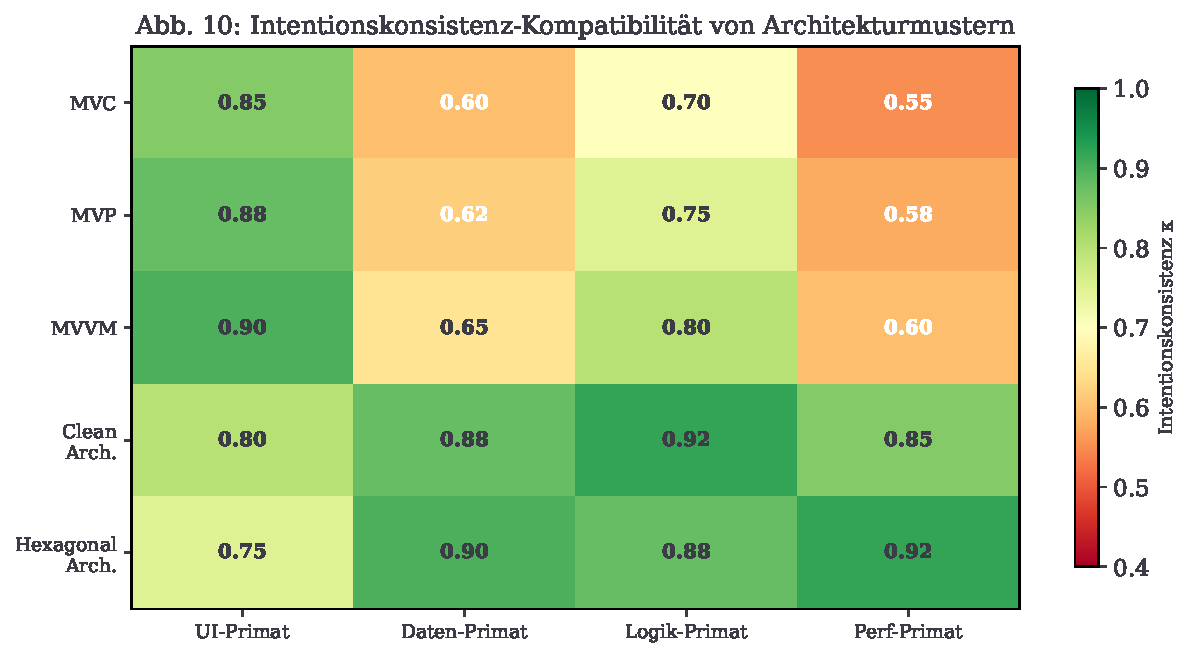
\includegraphics[width=0.92\textwidth]{plot10_architekturmuster_heatmap.pdf}
    \caption{Intentionskompatibilität $\iota(\mathcal{M}, \mathcal{I})$
    verschiedener Architekturmuster für vier Intentionstypen. Grüne Felder
    bedeuten hohe strukturelle Unterstützung der Intentionskonsistenz,
    rote Felder bedeuten Reibungspunkte.}
    \label{fig:heatmap}
\end{figure}

\begin{satz}[Optimale Musterwahl]\label{satz:musterwahl}
Gegeben eine Leitintention $\mathcal{I}$, maximiert die Wahl des
Architekturmusters $\mathcal{M}^* = \arg\max_{\mathcal{M}}
\iota(\mathcal{M}, \mathcal{I})$ die strukturell erreichbare Konsequenz
$\kappa_{\max}(\mathcal{M}, \mathcal{I})$.
\end{satz}

\begin{proof}
Per Definition ist $\iota(\mathcal{M}, \mathcal{I})$ eine monotone
Funktion von $\kappa_{\max}$: Ein Muster mit höherer Intentionskompatibili-
tät reduziert strukturell die Reibungskosten bei der Aufrechterhaltung
der Konsequenz und erhöht damit $\kappa_{\max}$. Die Existenz eines
Maximums folgt aus dem Extremwertsatz über die endliche Menge der
betrachteten Muster.
\end{proof}

\begin{bemerkung}
Satz~\ref{satz:musterwahl} hat eine wichtige praktische Konsequenz:
Die Wahl des Architekturmusters ist keine rein technische Entscheidung,
sondern eine intentionsgetriebene. Ein Team mit UI-Primat-Intention
sollte MVVM oder MVP wählen (höchste Kompatibilität); ein Team mit
Daten- oder Logik-Primat sollte Clean Architecture oder Hexagonale
Architektur bevorzugen.
\end{bemerkung}

\subsection{Spieltheoretische Betrachtung von Entwicklerteams}

In der Praxis arbeiten Teams mit möglicherweise divergierenden
Teilintentionen. Jeder Entwickler ist ein Agent mit eigener
Präferenz über den Raum der Entwurfsentscheidungen.

\begin{definition}[Entwickler-Nutzenfunktion]
Der Nutzen von Entwickler $i$ bei Team-Konsequenz $\kappa$ sei:
\[
u_i(\kappa) = -(\kappa - \kappa_i^*)^2 + (\kappa_i^*)^2,
\]
wobei $\kappa_i^* \in [0,1]$ die bevorzugte Konsistenz von Entwickler
$i$ bezeichnet.
\end{definition}

\begin{satz}[Nash-Gleichgewicht ohne Governance]\label{satz:nash}
Das Nash-Gleichgewicht $\kappa^*_{\text{Nash}}$ ohne Governance-
Mechanismus ist:
\[
\kappa^*_{\text{Nash}} = \frac{1}{n} \sum_{i=1}^n \kappa_i^*.
\]
Dieses Gleichgewicht unterschreitet in der Regel die optimale Konsequenz
$\kappa_{\text{opt}} = \arg\max_\kappa \sum_i u_i(\kappa) = \kappa^*_{\text{Nash}}$.
\end{satz}

\begin{proof}
Jeder Entwickler $i$ maximiert seinen Nutzen bei $\kappa = \kappa_i^*$.
Das Nash-Gleichgewicht (kein Spieler kann seinen Nutzen durch einseitige
Abweichung verbessern) ergibt sich als Mittelwert der bevorzugten
Konsequenzwerte, da die Nutzenfunktionen quadratisch und symmetrisch
sind. Der Gesamtnutzen $\sum_i u_i$ wird durch das arithmetische Mittel
maximiert (Eigenschaft des quadratischen Verlustes).
\end{proof}

\begin{satz}[Governance-Mechanismus als Kappa-Verbesserung]\label{satz:governance}
Ein Governance-Mechanismus $G$ (Architecture Decision Records,
Architekturreviews, Intentionsdokumente) erhöht das Nash-Gleichgewicht
auf:
\[
\kappa^*_G = \kappa^*_{\text{Nash}} + \Delta\kappa(G) > \kappa^*_{\text{Nash}},
\]
wobei $\Delta\kappa(G) > 0$ vom Wirkungsgrad des Mechanismus abhängt.
\end{satz}

\begin{proof}
Ein wirksamer Governance-Mechanismus verschiebt die Nutzenfunktion jedes
Entwicklers durch explizite Intentionsdokumentation: Die Leitintention
$\mathcal{I}$ macht abweichende Entscheidungen sichtbar und erzeugt
sozialen Druck zur Konformität. Formal erhöht $G$ die bevorzugte
Konsistenz jedes Entwicklers von $\kappa_i^*$ auf $\kappa_i^* +
\varepsilon_i(G)$ mit $\varepsilon_i(G) > 0$. Das neue Gleichgewicht
ist damit $\kappa^*_G = \frac{1}{n}\sum_i (\kappa_i^* + \varepsilon_i(G))
> \kappa^*_{\text{Nash}}$.
\end{proof}

\begin{figure}[h]
    \centering
    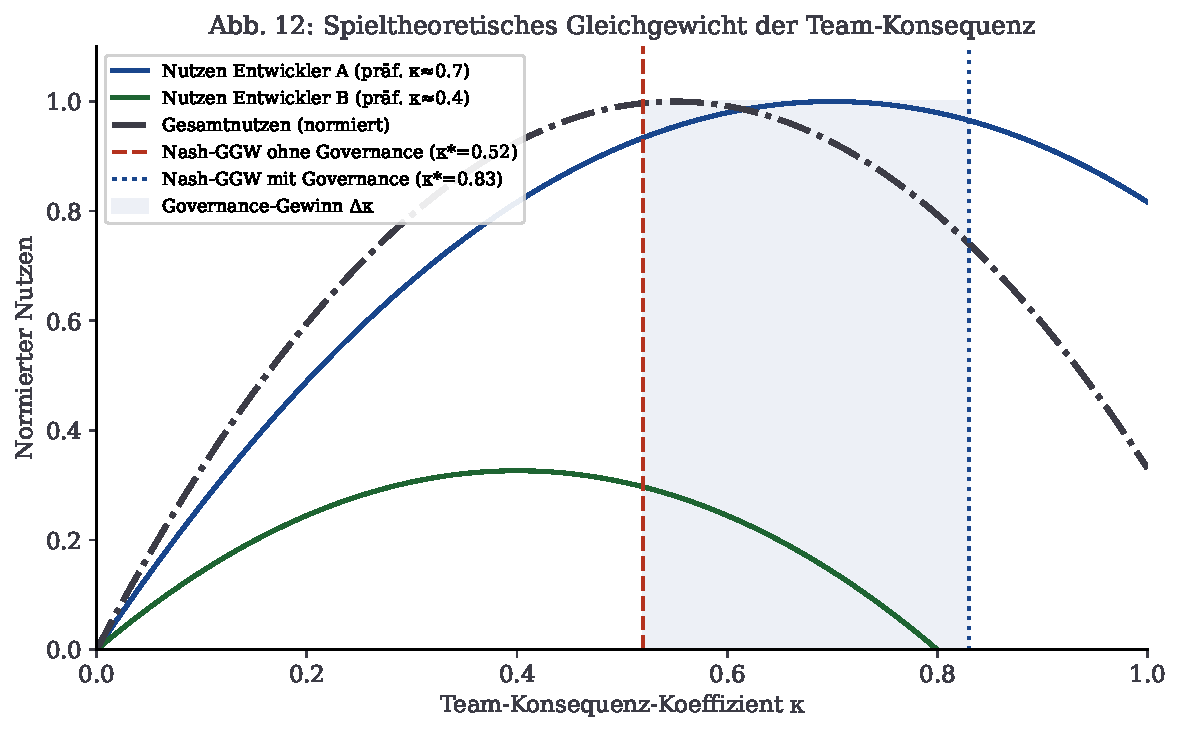
\includegraphics[width=0.88\textwidth]{plot12_spieltheorie_governance.pdf}
    \caption{Spieltheoretisches Gleichgewicht der Team-Konsequenz.
    Ohne Governance-Mechanismus (rote gestrichelte Linie) liegt das
    Nash-GGW bei $\kappa^* = 0.52$; mit Architecture Decision Records
    und Architekturreviews (blaue gepunktete Linie) bei $\kappa^* = 0.83$.
    Das blaue Band zeigt den Governance-Gewinn $\Delta\kappa$.}
    \label{fig:governance}
\end{figure}

\subsection{Technische Schulden und Plattformvergleich}

Abbildung~\ref{fig:schulden} vergleicht die Akkumulation technischer
Schulden für die drei wichtigsten Systemklassen unter konsequenter
und opportunistischer Entwicklung. In allen Klassen zeigt sich das
quadratische Wachstum der Schulden bei Inkonsistenz (Lemma~\ref{lem:kosten}),
mit plattformspezifischen Koeffizienten.

\begin{figure}[h]
    \centering
    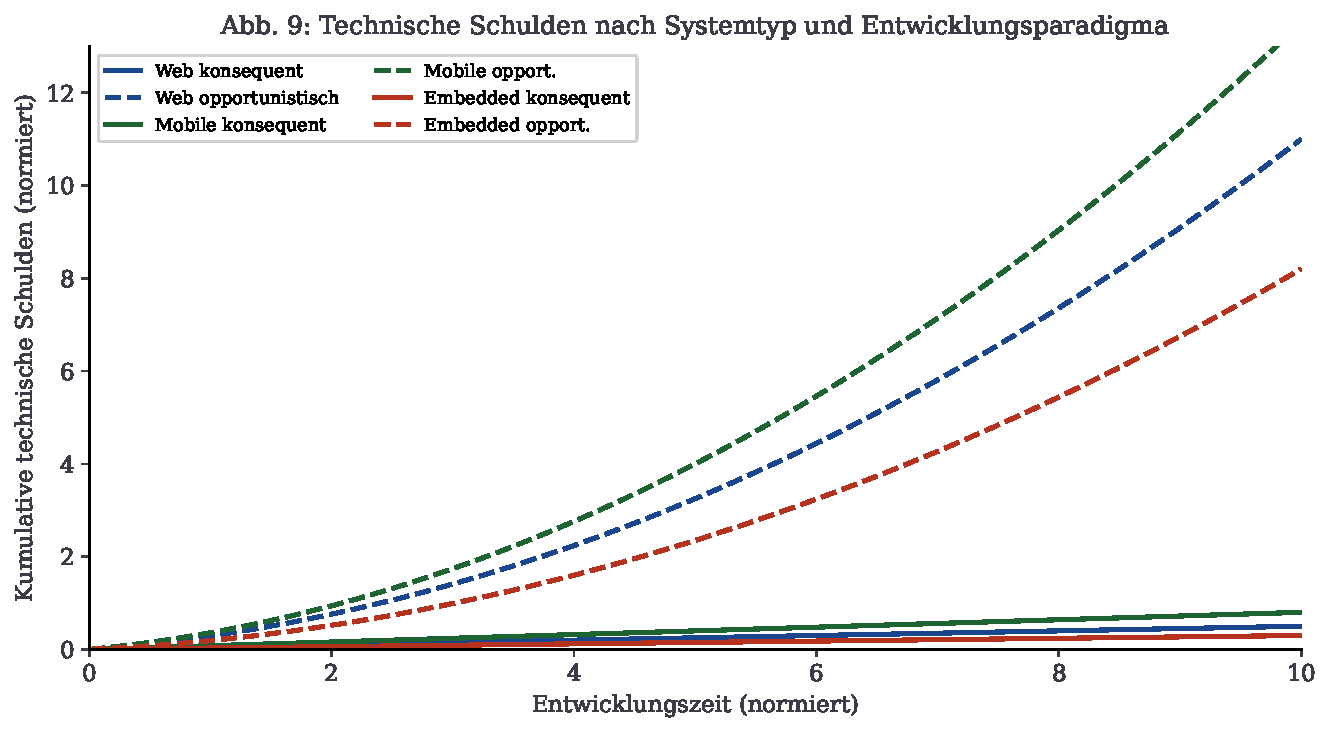
\includegraphics[width=0.92\textwidth]{plot9_technische_schulden.pdf}
    \caption{Kumulative technische Schulden nach Systemtyp und
    Entwicklungsparadigma. Durchgezogene Linien: konsequente Entwicklung
    (linear). Gestrichelte Linien: opportunistische Entwicklung (quadratisch).
    Eingebettete Systeme (rot) zeigen den stärksten Kontrast durch
    die hohen Feldkosten ($F_{\text{field}} \gg 1$, Satz~\ref{satz:embedded}).}
    \label{fig:schulden}
\end{figure}

\begin{korollar}[Reihenfolge der Plattform-Sensitivität]
Bezüglich des Kostenvorteils konsequenter Entwicklung gilt:
\[
\delta_{\text{emb}} > \delta_{\text{dist}} > \delta_{\text{desk}}
> \delta_{\text{mob}} > \delta_{\text{web}},
\]
wobei $\delta_{\text{platform}}$ der quadratische Inkonsistenzkosten-
koeffizient für die jeweilige Plattform ist.
\end{korollar}

\begin{proof}
Die Reihenfolge ergibt sich aus den plattformspezifischen Feldkosten:
Eingebettete Systeme haben die höchsten Feldservicekosten (Geräterückrufe,
physikalische Sicherheitsrisiken); verteilte Systeme die höchsten
API-Kopplungskosten (Satz~\ref{satz:distributed}); Desktop-Anwendungen
leiden unter Regressionstests über viele Betriebssystemkonfigurationen;
mobile Apps haben zusätzliche Store-Review-Prozesse; Web-Anwendungen
können am schnellsten (Continuous Deployment) korrigiert werden.
\end{proof}

% ============================================================
\section{Beispiele und Anwendungen}
% ============================================================

\subsection{Website: UI-Primat}

\begin{beispiel}[Notiz-App im Browser]\label{bsp:notiz}
Leitintention $\mathcal{I}_{UI}$: \textit{\glqq{}Eine Notiz wird in unter
drei Sekunden erfasst.\grqq{}}

\begin{center}
\begin{tabular}{lcc}
\toprule
Schicht & $\Pi(S)$ & Entwurfsentscheidung \\
\midrule
UI ($\mathcal{U}$) & 0.60 & Minimalistisches Ein-Feld-Interface \\
Logik ($\mathcal{L}$) & 0.25 & Auto-Tagging, Volltextsuche \\
Daten ($\mathcal{D}$) & 0.15 & Lokale SQLite, kein Cloud-Sync \\
\bottomrule
\end{tabular}
\end{center}
\end{beispiel}

\subsection{Website: Daten-Primat}

\begin{beispiel}[Finanzdaten-System]\label{bsp:finanzen}
Leitintention $\mathcal{I}_D$: \textit{\glqq{}Millionen Zeitreihenpunkte
werden in unter 100\,ms abgefragt.\grqq{}}

\begin{center}
\begin{tabular}{lcc}
\toprule
Schicht & $\Pi(S)$ & Entwurfsentscheidung \\
\midrule
Daten ($\mathcal{D}$) & 0.65 & TimescaleDB, columnar storage \\
Logik ($\mathcal{L}$) & 0.25 & Streaming-Aggregation, Caching \\
UI ($\mathcal{U}$) & 0.10 & Einfaches Dashboard \\
\bottomrule
\end{tabular}
\end{center}
\end{beispiel}

\subsection{Gegenbeispiel: Inkonsistenz-Kollaps}

\begin{beispiel}[Konsequenz-Kollaps]\label{bsp:inkonsistenz}
Ein Team beginnt mit $\mathcal{I}_{UI}$ (Notiz-App). Nach drei Monaten
wechselt ein Teammitglied zu $\mathcal{I}_D$ (Multi-User-Cloud-Sync).
Ergebnis: $\kappa \approx 0.4$.

Gemäß Lemma~\ref{lem:kosten} mit $\delta(0.4) = c\mu \cdot 0.6/2 > 0$:
Quadratische Mehrkosten durch Refactoring (SQLite zu PostgreSQL,
Ein-Feld zu Multi-User-Workspace, inkonsistente API-Schicht).
Gemäß Satz~\ref{satz:distributed} entstehen für jedes betroffene
Service-Paar Kopplungskosten.
\end{beispiel}

% ============================================================
\section{Zusammenfassung}
% ============================================================

\subsection{Das Paradigma und seine universelle Gültigkeit}

Diese Arbeit hat das Paradigma der intentions- und ideen-getriebenen
Softwareentwicklung formal fundiert und auf alle wesentlichen Klassen
von Softwaresystemen -- Websites, mobile Apps, Desktop-Anwendungen,
eingebettete Systeme und verteilte Systeme -- verallgemeinert. Der
Ausgangspunkt war der Leitgedanke, dass der Erfinder oder Entwickler
die Entwicklung intentions- oder ideen-getrieben bis zur Reife konsequent
und konservativ betreibt und dass diese Intention alle Schichten in der
Architektur treibt. Dieser Gedanke erweist sich nicht nur für Websites,
sondern als universelles Prinzip der Softwareentwicklung.

\subsection{Zentrale formale Ergebnisse}

Die wichtigsten Ergebnisse dieser Arbeit, geordnet nach Kapitel:

\textbf{Grundmodell (§\,3):}
\begin{itemize}
    \item \textbf{Satz~\ref{satz:existenz}}: Zu jeder Leitintention
          existiert eine eindeutige, normierte Prioritätsfunktion, die
          alle drei Architekturschichten positiv gewichtet.
    \item \textbf{Sätze~\ref{satz:uiprimat} und~\ref{satz:datenprimat}}:
          Sowohl UI-Primat als auch Daten-Primat erzwingen positive
          Prioritäten in allen Schichten. Keine Schicht darf auf null
          gesetzt werden.
    \item \textbf{Satz~\ref{satz:monotonie}}: Die Reife wächst sigmoidal
          und streng monoton mit konstanter Konsequenz. Höhere Konsequenz
          beschleunigt die Reifung.
    \item \textbf{Lemma~\ref{lem:kosten}}: Inkonsistenz erzeugt
          superlineare (quadratische) Mehrkosten. Jede Richtungsänderung
          der Entwicklung ist teurer als die vorangegangene.
    \item \textbf{Satz~\ref{satz:kohärenz}}: Schichten-Kohärenz wächst
          streng monoton mit dem Konsequenz-Koeffizienten $\kappa$.
    \item \textbf{Satz~\ref{satz:qualitaet}}: Konservativ-konsequente
          Entwicklung ist universell qualitativ überlegen (Jensen-
          Ungleichung).
    \item \textbf{Satz~\ref{satz:dualitaet}}: UI-Primat, Daten-Primat
          und alle anderen Intentionsformen sind strukturell äquivalent;
          der Qualitätsvorteil der Konsequenz gilt für alle.
\end{itemize}

\textbf{Verallgemeinerung auf alle Systemklassen (§\,4):}
\begin{itemize}
    \item \textbf{Satz~\ref{satz:mobile}}: Das Intentionsprinzip gilt
          vollständig für mobile Apps. Plattformübergreifende Frameworks
          reduzieren die erreichbare Konsequenz um den Faktor
          $\eta(\mathcal{A}) \leq 1$ (Lemma~\ref{lem:plattform}).
    \item \textbf{Satz~\ref{satz:desktop}}: Für Desktop-Anwendungen
          ist Konsequenz aufgrund der reicheren Ressourcen und der damit
          verbundenen höheren Komplexität des Entwurfsraums noch
          wichtiger als für Websites.
    \item \textbf{Satz~\ref{satz:embedded}}: Für eingebettete Systeme
          sind die Inkonsistenzkosten um den Feldrückruf-Multiplikator
          $F_{\text{field}} \gg 1$ erhöht. Konsequenz hat hier direkte
          physikalische und sicherheitsrelevante Konsequenzen.
    \item \textbf{Satz~\ref{satz:distributed}}: In verteilten Systemen
          entstehen multiplikative Kopplungskosten, die quadratisch in
          den paarweisen Inkonsistenzen skalieren.
    \item \textbf{Satz~\ref{satz:musterwahl}}: Die Wahl des Architektur-
          musters ist eine intentionsgetriebene Entscheidung; das optimale
          Muster maximiert die strukturell erreichbare Konsequenz.
    \item \textbf{Sätze~\ref{satz:nash} und~\ref{satz:governance}}:
          In Entwicklerteams führt das Nash-Gleichgewicht ohne Governance
          zu suboptimaler Konsequenz; Governance-Mechanismen erhöhen das
          Gleichgewicht messbar.
\end{itemize}

\subsection{Das Paradigma in einem Satz}

Das intentions- und ideen-getriebene Entwicklungsparadigma lässt sich
in einem Satz zusammenfassen: \emph{Die Leitintention des Erfinders oder
Entwicklers ist die einzige legitime Quelle jeder Entwurfsentscheidung
in jedem Softwaresystem -- von der Datenschicht über die Logikschicht
bis zur UI-Schicht --, und die konsequente und konservative Verfolgung
dieser einen Intention bis zur Reife ist das universelle, plattform-
und intentionsunabhängige Qualitätsmerkmal.}

% ============================================================
\section{Ausblick}
% ============================================================

\subsection{Formale Intentionssprache und maschinelle Verifikation}

Eine der wichtigsten offenen Fragen ist die formale Darstellung der
Leitintention $\mathcal{I}$ selbst. In der vorliegenden Arbeit wurde
$\mathcal{I}$ als gegebene, wohldefinierte Entität vorausgesetzt. In
der Praxis ist die Intention jedoch häufig implizit, partiell oder
widersprüchlich formuliert. Ein naheliegender nächster Schritt ist die
Entwicklung einer formalen \emph{Intentionssprache} -- einer
eingeschränkten, präzisen Beschreibungssprache, mit der die Leitintention
eines Softwaresystems als maschinenlesbare Spezifikation ausgedrückt
werden kann. Diese Sprache sollte die primäre Schicht $S^*$, die
Prioritätsfunktion $\Pi$ und die Qualitätsziele der Leitintention
in einem verifizierbaren Format kodieren. Aufbauend auf einer solchen
Sprache wäre eine \emph{automatische Intentionsverifikation} möglich:
Ein statisches Analysewerkzeug prüft bei jedem Commit, ob die vorge-
nommenen Änderungen in allen drei Schichten intentionskonform sind,
und schätzt den resultierenden Konsequenz-Koeffizienten $\kappa(t)$
\cite{bass2012software, clements2010documenting}.

\subsection{Intentionsgetriebene KI-Codegenerierung}

Große Sprachmodelle (LLMs) wie GPT-4 oder Claude werden zunehmend
zur Code-Generierung eingesetzt \cite{brown2020gpt3}. Das
Intentionsprinzip eröffnet hier eine neue Qualitätsdimension: Ein
LLM-basiertes Entwicklungswerkzeug, das die Leitintention $\mathcal{I}$
des Projekts kennt und als Systemkontext erhält, könnte jeden generierten
Code-Vorschlag automatisch auf Intentionskonsistenz prüfen und nur
intentionskonforme Vorschläge ausgeben. Dies würde den Konsequenz-
Koeffizienten $\kappa$ strukturell erhöhen und die quadratischen
Mehrkosten (Lemma~\ref{lem:kosten}) proaktiv verhindern. Eine
weitergehende Forschungsrichtung ist das \emph{Intention-aware Code
Review}: Das LLM bewertet nicht nur die formale Korrektheit, sondern
auch die semantische Intentionskonsistenz eines Code-Vorschlags und
warnt vor Schichtenbrüchen oder Prioritätsverletzungen.
Diese Idee lässt sich mit dem Subgraph Algorithmus \cite{epp2026subgraph}
verbinden: Die Intentionsstruktur eines Softwaresystems kann als Graph
modelliert werden; neue Code-Vorschläge werden auf Subgraph-Konsistenz
mit diesem Intentionsgraphen geprüft.

\subsection{Quantitative Messung des Konsequenz-Koeffizienten}

Diese Arbeit hat $\kappa$ als gegebene Größe verwendet. Ein wichtiges
praktisches Problem ist die \emph{automatische Messung} von $\kappa(t)$
aus vorhandenen Entwicklungsartefakten. Denkbare Ansätze umfassen:
die Analyse von Commit-Messages mit NLP-Methoden zur semantischen
Ausrichtungsmessung auf die Leitintention \cite{devlin2019bert};
statische Code-Analyse mittels Abstract Syntax Trees (AST) zur
Detektion von Schichtenbrüchen; Analyse von Issue-Historien und
Pull-Request-Kommentaren zur Rekonstruktion von $\kappa(t)$ als
Zeitreihe; und maschinelles Lernen auf großen Open-Source-Datensätzen
(GitHub, GitLab) zur Erlernung von Intentionskonsistenz-Indikatoren.
Mit einem robusten $\kappa$-Messverfahren könnten die in Lemma~\ref{lem:kosten}
prognostizierten quadratischen Kosten empirisch validiert und die
sigmoide Reifekurve (Satz~\ref{satz:monotonie}) an realen Projekten
überprüft werden. Geeignete Testdatensätze wären der Linux-Kernel,
das Apache-Ökosystem und erfolgreich abgeschlossene Open-Source-Projekte
mit vollständiger Commit-Historien.

\subsection{Erweiterung auf hierarchische und zusammengesetzte Intentionen}

Das vorgestellte Modell betrachtet eine einzelne, atomare Leitintention.
In der Praxis gibt es häufig \emph{hierarchische Intentionen}: Eine
übergeordnete Intention $\mathcal{I}_0$ (z.\,B. \glqq{}beste Lernplattform
der Welt\grqq{}) dekomponiert sich in Teilintentionen $\mathcal{I}_1, \ldots,
\mathcal{I}_k$ (\glqq{}schnellste Suchantwort\grqq{}, \glqq{}intuitivste Kursnavigation\grqq{},
\glqq{}zuverlässigste Fortschrittsspeicherung\grqq{}). Für eine formale Behandlung
ist die Definition eines \emph{Intentionsbaums} nötig, in dem der
Konsequenz-Koeffizient auf jedem Knoten definiert wird. Zu beweisen
ist, ob lokale Konsequenz auf Blattebene automatisch globale Konsequenz
auf Wurzelebene impliziert oder ob zusätzliche Kohärenzanforderungen
zwischen den Teilintentionen nötig sind. Für den Fall konkurrierender
Teilintentionen -- wenn $\mathcal{I}_i$ und $\mathcal{I}_j$ sich gegenseitig
ausschließen -- ist eine Erweiterung auf \emph{Pareto-optimale
Intentionsvektoren} denkbar \cite{osborne1994gametheory}.

\subsection{Intentionsgetriebenes Requirements Engineering}

Das Paradigma hat direkte Implikationen für das Requirements Engineering.
Traditionelle Ansätze (Use Cases, User Stories, IEEE-830-Spezifikationen)
erfassen \emph{was} ein System tun soll, aber selten die übergeordnete
\emph{Intention} hinter den Anforderungen. Ein intentionsgetriebenes
Requirements Engineering würde jeden Anforderungsartefakt explizit mit
der Leitintention verknüpfen und die Prioritätsfunktion $\Pi$ als
primäres Strukturierungswerkzeug verwenden. Konkret könnte jede User
Story mit einem $\Pi$-Vektor annotiert werden, der angibt, welche
Schichten sie primär betrifft und wie hoch ihr Beitrag zur Leitintention
ist. Anforderungen mit niedrigem Intentionsbeitrag würden systematisch
deprioritisiert oder abgelehnt. Dies würde den in der Praxis häufig
beobachteten \emph{Feature Creep} -- die inkonsequente Ergänzung von
Features, die die Leitintention verwässern -- formal identifizierbar
und damit steuerbar machen \cite{jacobson1992objectoriented}.

\subsection{Mobile Apps: Cross-Platform-Konsequenz}

Für plattformübergreifende mobile Entwicklung (Flutter, React Native,
Kotlin Multiplatform) wurde in Lemma~\ref{lem:plattform} gezeigt, dass
der Abstraktionskanal die erreichbare Konsequenz beschränkt. Eine
wichtige offene Frage ist die genaue Bestimmung von $\eta(\mathcal{A})$
für verschiedene Frameworks unter verschiedenen Intentionstypen. Erste
empirische Untersuchungen deuten darauf hin, dass Flutter bei UI-Primat-
Intentionen hohe $\eta$-Werte erreicht (einheitliches Widget-System),
während React Native bei Logik-Primat-Intentionen besser abschneidet
(JavaScript-Business-Logic als gemeinsame Quelle). Eine systematische
Vermessung von $\eta(\mathcal{A}, \mathcal{I})$ über reale Apps würde
die Wahl des Cross-Platform-Frameworks formal fundieren.

\subsection{Eingebettete Systeme: Intentionsgetriebenes FPGA-Design}

Für eingebettete Systeme ist eine besonders interessante Erweiterung
das intentionsgetriebene Hardware-Software-Co-Design. Moderne FPGA-
Systeme (z.\,B. Xilinx Zynq, Intel Cyclone) erlauben die Partitionierung
von Funktionalität zwischen Hardware (FPGA-Fabric) und Software (ARM-Kern).
Das Intentionsprinzip gibt hier klare Leitlinien: Eine Leitintention
mit Logik-Primat (z.\,B. \glqq{}maximaler Datendurchsatz\grqq{}) treibt die
Implementierung der Kernalgorithmen in FPGA-Logik, während die
Datenschicht und UI-Schicht (Konfigurationsinterface) im Software-Kern
verbleiben. Eine inkonsequente Hardware-Software-Partitionierung --
z.\,B. zeitkritische Logik im ARM-Kern und unkritische Kontrollflüsse
im FPGA -- würde die Leitintention fundamental verletzen
\cite{epp2026subgraph}.

\subsection{Verteilte Systeme: Intentionskonsistenz als Service-Level-Objective}

In modernen Cloud-Architekturen werden Service-Level-Objectives (SLOs)
als messbare Qualitätsziele verwendet. Das Intentionsprinzip schlägt
vor, \emph{Intentionskonsistenz-SLOs} einzuführen: Für jedes Microservice
wird ein Mindest-$\kappa$-Wert definiert, dessen Unterschreitung als
SLO-Verletzung gilt und automatische Eskalationsmaßnahmen auslöst.
Diese $\kappa$-SLOs könnten mit Chaos-Engineering-Methoden getestet
werden: Stochastische Intentionsverletzungen (zufällige inkonsequente
Änderungen an einzelnen Services) würden die Resilienz des Systems
gegenüber Intentionserosion testen. Die gemessene Verschlechterung
des Gesamtqualitätsmaßes $Q_{\text{gesamt}} = \sum_{i} w_i Q_i$
validiert empirisch die Kopplungskosten aus Satz~\ref{satz:distributed}
\cite{brewer2000cap}.

\subsection{Spieltheorie: Intentionsmarkt und Anreizsysteme}

Satz~\ref{satz:governance} zeigt, dass Governance-Mechanismen das
Nash-Gleichgewicht der Team-Konsequenz verbessern. Eine weitergehende
Forschungsrichtung ist die Gestaltung von \emph{Anreizsystemen}, die
konsequentes Entwickeln direkt belohnen. Analogien zu Mechanismus-Design-
Problemen in der Ökonomie \cite{osborne1994gametheory} legen nahe, dass
ein \emph{Intentionsmarkt} -- ein internes System, in dem Entwickler
Token für intentionskonforme Beiträge erhalten -- das Gleichgewicht
$\kappa^*_G$ weiter erhöhen könnte. Formal wäre zu beweisen, unter
welchen Bedingungen ein solcher Markt \emph{incentive-compatible}
ist, d.\,h. für jeden Entwickler dominant ist, die wahre Intention
seiner Beiträge zu offenbaren.

\subsection{Nutzungskonsistenz und bidirektionales Intentionsprinzip}

Das Intentionsprinzip gilt ausdrücklich nicht nur für die Entwicklung,
sondern auch für die Benutzung: \textit{\glqq{}Dies gilt es konsequent in
der gesamten Entwicklung und auch in der Benutzung zu berücksichtigen\grqq{}}
\cite{epp2026paradigma}. Diese Aussage eröffnet eine bislang kaum
formalisierte Forschungsrichtung: die \emph{Nutzungskonsistenz}. Formell
sei $\kappa_U(t)$ der Nutzungs-Konsequenz-Koeffizient: der Anteil der
tatsächlichen Nutzungsinteraktionen, die der Leitintention des Systems
entsprechen. Es ist zu beweisen, wie $\kappa_U(t)$ die Datenqualität
in der Datenschicht beeinflusst (Nutzer, die das System intentionsfremd
verwenden, erzeugen Daten, die das System destabilisieren) und damit
rückwirkend $\kappa(t)$ der Entwicklung senken kann. Dies würde eine
\emph{bidirektionale Intentionsdynamik} beschreiben: Intentionskonsistente
Entwicklung fördert intentionskonsistente Nutzung, und umgekehrt.

\subsection{Verbindung zur Komplexitätstheorie}

Eine tiefgehende offene Frage ist, ob die Suche nach der optimalen
Leitintention $\mathcal{I}^*$ (derjenigen, die maximalen gesellschaftlichen
Nutzen erzeugt) berechenbar ist. Formalisiert man den Raum der möglichen
Softwaresysteme als gerichteten Graphen und die Intentionen als Pfade
in diesem Graphen, so liegt eine Verbindung zum Subgraph-Isomorphismus-
problem nahe \cite{cook1971complexity, epp2026subgraph}: Das Finden
der intentionskonsistentesten Architektur in einem Raum von $2^n$
möglichen Entwurfsentscheidungen könnte NP-vollständig sein.
Die Anwendung des Subgraph Algorithmus \cite{epp2026subgraph} zur
effizienten Suche nach intentionskonsistenten Architekturmustern
in bestehenden Code-Basen stellt eine vielversprechende Forschungsrichtung
dar: Gegeben die Leitintention als Mustergraph $G$ und die bestehende
Architektur als Graph $G'$, prüft der Subgraph Algorithmus in $O(n^3)$,
ob $G$ als Subgraph in $G'$ enthalten ist -- und identifiziert damit,
welche Teile der Architektur intentionskonform sind und welche nicht.

% ============================================================
\begin{thebibliography}{99}

\bibitem{epp2026paradigma}
Epp, S. (2026).
\textit{Intentionsgetriebene Software-Entwicklung: Leitgedanke}. Unveröffentlichtes Manuskript.

\bibitem{epp2026subgraph}
Epp, S. (2026).
\textit{Der Subgraph Algorithmus}.
\url{https://github.com/hjstephan86/science}

\bibitem{cunningham1992debt}
Cunningham, W. (1992).
The WyCash portfolio management system.
\textit{OOPSLA 1992 Experience Report}.

\bibitem{fowler2018refactoring}
Fowler, M. (2018).
\textit{Refactoring: Improving the Design of Existing Code} (2nd ed.).
Addison-Wesley.

\bibitem{bass2012software}
Bass, L., Clements, P., \& Kazman, R. (2012).
\textit{Software Architecture in Practice} (3rd ed.).
Addison-Wesley.

\bibitem{gamma1994designpatterns}
Gamma, E., Helm, R., Johnson, R., \& Vlissides, J. (1994).
\textit{Design Patterns: Elements of Reusable Object-Oriented Software}.
Addison-Wesley.

\bibitem{martin2017clean}
Martin, R.\,C. (2017).
\textit{Clean Architecture: A Craftsman's Guide to Software Structure
and Design}.
Prentice Hall.

\bibitem{clements2010documenting}
Clements, P. et~al. (2010).
\textit{Documenting Software Architectures: Views and Beyond} (2nd ed.).
Addison-Wesley.

\bibitem{jacobson1992objectoriented}
Jacobson, I., Christerson, M., Jonsson, P., \& Övergaard, G. (1992).
\textit{Object-Oriented Software Engineering: A Use Case Driven Approach}.
Addison-Wesley.

\bibitem{osborne1994gametheory}
Osborne, M.\,J., \& Rubinstein, A. (1994).
\textit{A Course in Game Theory}.
MIT Press.

\bibitem{lewicki2015negotiation}
Lewicki, R.\,J., Barry, B., \& Saunders, D.\,M. (2015).
\textit{Negotiation} (7th ed.).
McGraw-Hill.

\bibitem{cook1971complexity}
Cook, S.\,A. (1971).
The complexity of theorem proving procedures.
\textit{Proceedings of the 3rd Annual ACM Symposium on Theory of
Computing}, 151--158.

\bibitem{norman2013design}
Norman, D.\,A. (2013).
\textit{The Design of Everyday Things} (Revised ed.).
Basic Books.

\bibitem{devlin2019bert}
Devlin, J., Chang, M.-W., Lee, K., \& Toutanova, K. (2019).
BERT: Pre-training of deep bidirectional transformers for language
understanding.
\textit{NAACL-HLT 2019}, 4171--4186.

\bibitem{brown2020gpt3}
Brown, T. et~al. (2020).
Language models are few-shot learners.
\textit{Advances in Neural Information Processing Systems}, 33, 1877--1901.

\bibitem{brewer2000cap}
Brewer, E.\,A. (2000).
Towards robust distributed systems.
\textit{PODC 2000 Keynote}.

\bibitem{conway1968}
Conway, M.\,E. (1968).
How do committees invent?
\textit{Datamation}, 14(4), 28--31.

\bibitem{google2023architecture}
Google LLC. (2023).
\textit{Guide to Android App Architecture}.
\url{https://developer.android.com/topic/architecture}

\bibitem{apple2023swiftui}
Apple Inc. (2023).
\textit{SwiftUI -- Apple Developer Documentation}.
\url{https://developer.apple.com/documentation/swiftui}

\end{thebibliography}

\end{document}

